\documentclass[a4paper,11pt]{report}

%% subsubsubsection (\paragraph{})
\usepackage{titlesec}

\setcounter{secnumdepth}{4}

\titleformat{\paragraph}
{\normalfont\normalsize\bfseries}{\theparagraph}{1em}{}
\titlespacing*{\paragraph}
{0pt}{3.25ex plus 1ex minus .2ex}{1.5ex plus .2ex}


% Packages
\renewcommand{\baselinestretch}{1.5} 
% \renewcommand{\listfigurename}{List of plots} % Want to change "List of Figures" title ?
% \renewcommand{\listtablename}{Tables} % List of table ?
\usepackage{multirow} % Multi row row
\usepackage{fontspec}
\setmainfont[Path=calibri/,
    BoldItalicFont=calibriz.ttf,
    BoldFont      =calibrib.ttf,
    ItalicFont    =calibrii.ttf]{calibri.ttf}
\usepackage[english]{babel}
\addto\captionsenglish{% To change CONTENT title
  \renewcommand{\contentsname}%
    {TABLE OF CONTENTS}%
}

% Code
\usepackage{listings}

% Math
\usepackage{amsmath}

%% Images
\usepackage{graphicx} % Display images
\usepackage{float} % Image prositions
\graphicspath{ {images/} } % Path of the images folder
\usepackage{caption}
\usepackage{subcaption}
%%%%%%%%%

\usepackage{fancyhdr} % Header & footer
\usepackage{vmargin}
\usepackage{acronym} % list of abbreviations / acronyms
\usepackage{url} % Put urls
\usepackage{titlesec}
\usepackage{verbatim} % Multiline comment
\usepackage[export]{adjustbox} % Align images right / left
\usepackage[hidelinks]{hyperref} % Allow to click on citation
\hypersetup{ % Links style
    colorlinks=true,
    linkcolor=black,
    filecolor=magenta,      
    urlcolor=cyan,
}

% Disable auto indent
\setlength{\parindent}{0pt}

% Margins
\setmarginsrb{2.5 cm}{2.5 cm}{2.5 cm}{2.5 cm}{1 cm}{1 cm}{1 cm}{1 cm}
%1 left
%2 top
%3 right
%4 bottom
%5 header
%6 header and text
%7 footer
%8 footer and text

\title{\textsc{Cloud Computer Vision for Wildlife Monitoring}}
\author{\textsc{25313} - \textsc{2019}} % \textsc{Louis} \textsc{Beaumont}
\date{\today}

% Main variables
\makeatletter
\let\thetitle\@title
\let\theauthor\@author
\let\thedate\@date
\makeatother

% Header & Footer
\pagestyle{fancy}
\fancyhf{}
\rhead{\theauthor}
\lhead{Cloud Computer Vision for Wildlife Monitoring}
\cfoot{\thepage}

% Remove "Chapter N"
\titleformat{\chapter}[display]{\normalfont\bfseries}{}{0pt}{\Large}
\includeonly{title,acknowledgements,resume,abstract,introduction,computer-vision,related,implementation,future,automation,conclusion}
\begin{document}

%%%%%%%%%%%%%%%%%%%%%%%%%%%%%%%%%%%%%%%%%%%%%%%%%%%%%%%%%%%%%%%%%%%%%%%%%%%%%%%%%
%%%	Cover page
%%%%%%%%%%%%%%%%%%%%%%%%%%%%%%%%%%%%%%%%%%%%%%%%%%%%%%%%%%%%%%%%%%%%%%%%%%%%%%%%%

\begin{titlepage}
    \centering
    \vspace*{0.5 cm}
    %
\includegraphics[scale = 1]{ynov.png}\\[1.0 cm]  % University Logo
    \textsc{\Large Master 2 - Data science}\\[0.5 cm]     
    \rule{\linewidth}{0.2 mm} \\[0.4 cm]
    { \huge \bfseries \theauthor}\\
    \rule{\linewidth}{0.2 mm} \\[0.4 cm]
    { \huge \bfseries Annexes\\}%\thetitle}\\
    \rule{\linewidth}{0.2 mm} \\[1.5 cm]
\end{titlepage} % Cover

\chapter*{} % Epigraph
When the first humans reached Australia about 45,000 years ago, they quickly drove to extinction 90\% of its large animals. This was the first significant impact that Homo sapiens had on the planet's ecosystem. It was not the last.


― Yuval Noah Harari

%%%%%%%%%%%%%%%%%%%%%%%%%%%%%%%%%%%%%%%%%%%%%%%%%%%%%%%%%%%%%%%%%%%%%%%%%%%%%%%%%
% Thanks
%%%%%%%%%%%%%%%%%%%%%%%%%%%%%%%%%%%%%%%%%%%%%%%%%%%%%%%%%%%%%%%%%%%%%%%%%%%%%%%%%

\chapter{Acknowledgements}
\begin{it}



The past six months have been an exciting journey, dedicated to the last step in finishing my master Data Science at Ynov Aix-en-Provence: writing this thesis. I would like to express my sincere gratitude to those who helped me during this period.

First of all, I would like to thank Pascal Alanche for giving me the opportunity to work at Arpège SAS a Rohde \& Schwarz company during my 3 years of apprenticeship. It was a great experience to be part of the R\&D team and participate in the many interesting projects of the company. I have met a lot of remarkable people who taught me valuable knowledge about geostationary satellites and high-frequency radio communication. I would like to thank my supervisor from Ynov, Renaud Angles, for his guidance throughout the research project. His feedback, whether it was enthusiastic or critical, helped me to structure and improve this thesis and to continue the project at tough points.

Likewise, I would like to thank Olivier Gimenez, Oksana Grente, Anna Chaine, Lucile Marescot from the CNRS and ONCFS for their invaluable information about the context of camera-trap and wildlife monitoring, as well as the introduction to ecology research.

My gratitude also goes to the people of the open-source world from the people sharing publicly datasets, to the people on the algorithm side, developing amazing framework and making fantastic tutorials, thanks Github, Microsoft, Google, especially in my case at least.

Finally, I would like to express my gratitude to my parents and family for their support and wisdom throughout my thesis. Especially my brother Romain who guided me through the difficulties encountered on the technical parts.

I hope that you will enjoy reading the current research. If you have any questions or comments, please do not hesitate to contact me.

\end{it}

%%%%%%%%%%%%%%%%%%%%%%%%%%%%%%%%%%%%%%%%%%%%%%%%%%%%%%%%%%%%%%%%%%%%%%%%%%%%%%%%%
% Résumé en français
%%%%%%%%%%%%%%%%%%%%%%%%%%%%%%%%%%%%%%%%%%%%%%%%%%%%%%%%%%%%%%%%%%%%%%%%%%%%%%%%%

\chapter{Résumé}
Dans ce travail, je présente une solution hébergée dans le cloud facile à déployer, à maintenir, à mettre à l'échelle et à tarifer pour la surveillance de la faune à l'aide de l'intelligence artificielle, qui permet d'effectuer une vaste collecte et analyse de données et de déployer et suivre rapidement de nouvelles données de surveillance pour tout groupe particulier d'espèces et dans tout habitat. En particulier, je montre comment ce logiciel peut évoluer de quelques images initiales à des dizaines de milliers de vidéos par mois.

La surveillance de l'état des espèces de notre planète à l'aide d'une grande variété de technologies et de plateformes est cruciale pour améliorer la conservation de la biodiversité et pour développer de nouvelles méthodes de gestion des espèces. Je montre comment mettre en œuvre une application de surveillance de la faune directement dans le cloud à l'aide de l'intelligence artificielle (IA). Cette solution offre également des moyens d'analyser les données pour la surveillance des espèces et la capacité d'agréger les données afin d'identifier les modèles et les tendances pour informer les écologistes.

Plus important encore, pour l'identification des animaux, le système permet d'économiser un temps considérable de travail manuel tout en offrant le même niveau de précision que les bénévoles humains. % abstract in french ?

%%%%%%%%%%%%%%%%%%%%%%%%%%%%%%%%%%%%%%%%%%%%%%%%%%%%%%%%%%%%%%%%%%%%%%%%%%%%%%%%%
% Abstract
%%%%%%%%%%%%%%%%%%%%%%%%%%%%%%%%%%%%%%%%%%%%%%%%%%%%%%%%%%%%%%%%%%%%%%%%%%%%%%%%%

\chapter{Abstract}
In this work I present an easy to deploy, maintain, scale and price cloud solution for wildlife monitoring powered by artificial intelligence, which makes it possible to conduct an extensive data collection and analysis and to quickly deploy and track new monitoring data for any particular group of species and in any habitat. In particular, I show how this software can scale from an initial few images to up to tens of thousands of videos per month.

I believe that monitoring of the status of our planet's animals using a wide variety of technology and platforms is crucial to improve biodiversity conservation and to develop novel methods of managing species. I demonstrate how to implement a cloud application for cloud based monitoring of wildlife using artificial intelligence (AI). This solution also offer ways to analyze the data for the monitoring of species and the ability to aggregate data to identify patterns and trends to inform ecologists.

Most importantly, for animal identification, our system can save a tremendous amount of time of the manual labor while performing at the same accuracy level than human volunteers. % Whats this thing about in 1 page

\tableofcontents

% \listoftables

\listoffigures % List of figures ...

%%%%%%%%%%%%%%%%%%%%%%%%%%%%%%%%%%%%%%%%%%%%%%%%%%%%%%%%%%%%%%%%%%%%%%%%%%%%%%%%%
% Introduction
%%%%%%%%%%%%%%%%%%%%%%%%%%%%%%%%%%%%%%%%%%%%%%%%%%%%%%%%%%%%%%%%%%%%%%%%%%%%%%%%%

\chapter{Introduction}

The present work is intended, as far as possible, to give an insight into the process of automating cognitive task in the cloud to those readers who, from a general scientific and philosophical point of view, are interested in the field of artificial intelligence and ecology.


As the planet changes due to urbanization and climate change, biodiversity in the world is declining. We are currently witnessing an estimate of the increasing rate of species loss 200 times more than historical rates\cite{cop21_1}. 

The Earth's biodiversity is rapidly changing in what may be considered as one of the largest environmental challenges of our time.

For example, there is no doubt that in 2040 approximately one-third of all living species will be in the range of mammals living in the world today. How much of these new species will become endangered is unclear, and it might be impossible to assess exactly because there are still so many unknowns about the changes in our planet at large. There is no good data to guide us to any prediction for how our species will recover from the loss of species and how many we will need to lose to sustain human population growth of current levels.

At least for now, ecologists and volunteers are trying to collect such data but they spend a huge amount of time manually identifying species in images, in this era of digitization, something can be done.

Indeed, recent pattern recognition techniques allow computers to understand the semantics of images, allowing the automation of this cognitive task.


This subject is important, first, it has high practical relevance. The amount of time gained by automatizing manual labours is tremendous. Second, this study can be beneficial to the theory building in the emerging research field of deep learning and especially in the area of computer vision.

Furthermore, this work can be valuable for those interested in the field of big data and cloud computing, which grant an easy access to deploying, scaling and maintaining automated tasks.


This work includes several dimensions: 
\begin{itemize}
    \item Ecology: the balance of living being survival
    \item Artificial intelligence
    \item Big data \& cloud computing
\end{itemize}

We propose an architecture that is easy to deploy, use, maintain and price entirely in the cloud, allowing wildlife monitoring through concrete data visualisations.

Through this thesis, the answer to this question will be given:

\begin{it}  
How to automatize and scale wildlife monitoring using cloud computer vision ?
\end{it}


In this thesis, we first introduce the collaborators of this projects such as the ONCFS and CNRS.

Secondly, a short explanation of computer vision is stated.

We then mention the related work on computer vision and wildlife monitoring, especially the datasets available and existing algorithms.

Finally, the implementation done and the future possible work will be presented.

The answer to the problematic will then be discussed, followed by a conclusion.




\pagebreak\section{ONCFS}
the French National Office for Hunting and Wildlife aims to safeguard and sustainably manage wildlife and its habitats.
A public institution under the dual supervision of the Ministries of Ecology and Agriculture, the National Hunting and Wildlife Office fulfils five main missions responding to the main lines of the last Environmental Conference, following the Grenelle de l'Environnement:

territorial surveillance and the environment and hunting police,
studies and research on wildlife and its habitats,
technical support and advice to administrations, local authorities, managers and spatial planners,
the evolution of hunting practices in accordance with the principles of sustainable development and the development of environmentally friendly rural land management practices,
the organization of the examination and the issuance of the hunting permit. 
The ONCFS in a few figures
Created in 1972, the Office has a budget of 120 million euros to carry out its missions throughout the country (metropolitan France and the French overseas departments). 

1,700 people working for biodiversity:
\begin{itemize}
  \item 1,000 Environmental Technical Agents, commissioned by the Ministry in charge of sustainable development, divided into Departmental Services and Mobile Intervention Brigades
  \item 350 Environmental Technicians, also commissioned, assigned to Departmental Services (supervision), Inter-Regional Delegations and the various departments
  \item 70 engineers and technicians, grouped in five C.N.E.R.A. specialized in a group of species: migratory birds, deer and wild boars, mountain fauna, small sedentary plain fauna, predators and predatory animals.
  \item 80 technical managers
  \item 156 administrative staff
  \item 30 workers involved in the management of the domains and reserves managed or co-managed by the Office.
  \item 25 hunting licence inspectors
  \item 6 departments, in support of the Director General, implement the institution's action in their areas of competence
  \item 10 Inter-Regional Delegations - 90 Departmental Services
  \item 1 Board of Directors
  \item 1 Scientific Council
  \item 27 wildlife reserves, totalling nearly 60,000 hectares of protected areas that allow the ONCFS to carry out studies and experiments.
\end{itemize}

ONCFS brought useful information about camera-trap context, the animals monitored and provided a set of videos and images of camera-trap taken lynxes and wolves.

ONCFS could gain a lot of time from the solution presented in this thesis, without losing any accuracy compared to human-level animal detection.

\pagebreak\section{CNRS}

The Centre national de la recherche scientifique, better known by the acronym CNRS, is the largest French public scientific research organisation. Legally, it is a public scientific and technological institution (EPST) under the administrative supervision of the Ministry of Higher Education, Research and Innovation.

Founded by the Decree-Law of 19 October 19391, in order to "coordinate the activity of laboratories in order to obtain a higher return from scientific research", the CNRS was reorganized after the Second World War and then moved clearly towards fundamental research.

The CNRS operates in all fields of knowledge through a thousand accredited research and service units, most of which are managed with other structures (universities, other EPSTs, grandes écoles, industries, etc.) for five years in the administrative form of "mixed research units".


The CNRS was created on 19 October 1939, following the merger between an agency of resources, the Caisse nationale de la recherche scientifique and a major institution of laboratories and researchers, the Centre national de la recherche scientifique appliquée.

This merger was prepared by Jean Zay with the help of the Under-Secretaries of State for Research Irene Joliot-Curie and Jean Perrin. The decree organizing the CNRS is signed by the current President of the Republic, Albert Lebrun, the President of the Council, Édouard Daladier, the Minister of National Education, Yvon Delbos, succeeding Jean Zay, and the Minister of Finance, Paul Reynaud. The creation of the CNRS was intended to "coordinate the activity of laboratories in order to obtain a higher return from scientific research" and, in the words of Jean-François Picard, to "merge it into a single body, in a way the logical outcome of scientific and centralizing Jacobinism".

Fusion was encouraged by the Second World War: the French authorities, not wishing to reproduce the mistakes made during the First World War (all the scientists had been mobilized, often as executives in the infantry or artillery, which led to the disappearance of a high proportion of young scientists), assigned researchers to the CNRS. This merger therefore did not attract any press coverage. At the beginning, part of the research was conducted for the needs of the French army. Threatened by the Vichy Regime, which finally maintained it and confirmed geologist Charles Jacob6 at its head, the CNRS was reorganized at the Liberation. Frédéric Joliot-Curie was appointed director and provided him with new research grants.

De Gaulle's arrival in power in 1958 opened a period described as the "golden age of scientific research" and the CNRS: the CNRS' budget doubled between 1959 and 19628.

In 1966, associated units were created, ancestors of the UMRs. These are university laboratories, supported by the CNRS, thanks to its human and financial resources. In 1967, the National Institute of Astronomy and Geophysics was founded, which in 1985 became the National Institute of Universe Sciences (INSU). The National Institute for Nuclear and Particle Physics (IN2P3) was established in 1971.

In the 1970s, there was a change from science to society: the CNRS wondered about its ambition and its modes of action. The first interdisciplinary programmes are launched and global contracts with industry are signed (the first with Rhône-Poulenc in 1975).

In 1982, the law of 15 July, known as the Chevènement de programmation des moyens de la recherche publique law, decreed that research personnel, technical and administrative engineers and administrative staff are to be transferred to the civil service: they become civil servants, with, for researchers, a status similar to that of lecturers and university professors.

According to a survey conducted in 2009 by Sofres for Sciences Po, the CNRS enjoyed a 90\% level of trust among the French, well before the police (71\%), the Government (31\%), the President of the Republic (35\%) or political parties (23\%), and second only after the family (97\%).

The CNRS of Montpellier has been of great help, both in terms of additional information for cameras, but also in terms of research in the field of ecology and the kind of data that could potentially interest them...

\chapter{Computer vision}
With the rise of the Internet and modern technologies, we can now confirm with certainty that we live in an image-based society, the video sharing platform Youtube is responsible for 37\% of all mobile internet traffic alone (see Figure ~\ref{fig:youtube}).

\begin{figure}[H]
  \centering
  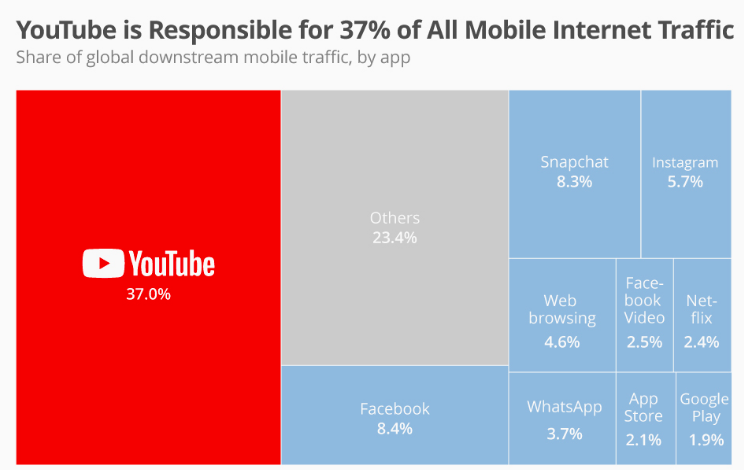
\includegraphics[width=.8\linewidth]{youtube_traffic.png}
  \caption{Youtube internet traffic share. \href{https://www.statista.com/chart/17321/global-downstream-mobile-traffic-by-app}{Source}}
  \label{fig:youtube}
\end{figure}

With about 3.5 billion smartphone users\cite{stats_smartphone_usage}, a huge part using massively visual content sharing platforms, the amount of information transmitted by this data is enormous, so automating the abstract information extraction of these pixels has an unimaginable potential.
Computer Vision is a technology that allows computers to extract abstract information from visual content.

\pagebreak\section{What is it}
The term "computer vision" refers to the different techniques that allow computers to see and understand the content of images. This is a sub-category of artificial intelligence and machine learning.

The computer vision field brings together multiple techniques from various fields of engineering or computer science. In general, the different methods aim to reproduce the human vision. To understand the content of images, machines must be able to extract a description: an object, a description, a 3D model...

Some computer vision systems may also require image processing, i.e. simplifying or augmenting the content of the image. Examples include normalizing the photo-metric properties of the image, cropping its contours or removing noise such as digital artifacts induced by low light.

\pagebreak\section{Challenges}

What could be simpler than vision? From birth, humans are naturally able to see. However, allowing a computer to do the same is not an easy task. To date, computer vision still fails to match human vision.

One of the reasons is that we still do not really know how human vision works. We need to understand how perceptual organs such as the eyes work, but also how the brain interprets this perception. Although research in this area is progressing at a rapid pace, we are still a long way from unlocking all the mysteries of vision.

Another challenge is related to the complexity of the visual world. An object can be perceived from multiple angles, under various lighting conditions, partial hidden by other objects...

A true computer vision system must be able to perceive the content in any of these situations and extract information from it. In fact, computer vision is a real scientific challenge.

\pagebreak\section{Deep learning}

Several years ago, most computer vision algorithms consisted of simple heuristics to extract features from pixels (See an example of heuristic on Figure ~\ref{fig:haar}).
\begin{figure}[H]
  \centering
  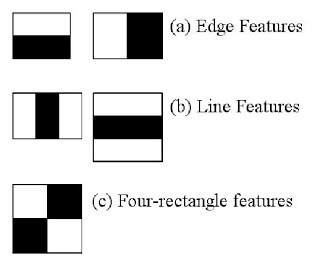
\includegraphics[width=.35\linewidth]{haar_classifier.jpg}
  \caption{Haar features. \href{https://towardsdatascience.com/learning-computer-vision-41398ad9941f}{Source}}
  \label{fig:haar}
\end{figure}
Over time, there has been more and more use of machine learning and such automatic pattern recognition algorithm, the true revolutionising technology that have made machine learning in general works so well is neural networks and especially deep neural networks (see Figure ~\ref{fig:deeplearning}).

\begin{figure}[H]
  \centering
  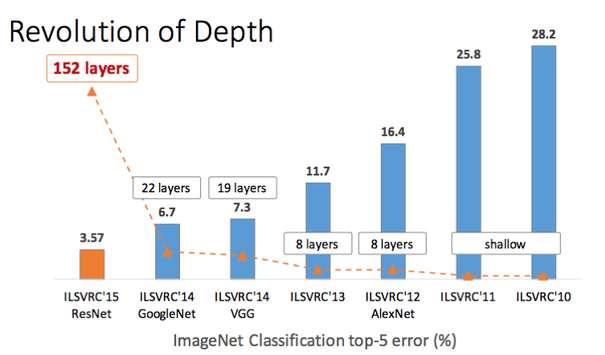
\includegraphics[width=.7\linewidth]{deep_learning.png}
  \caption{Revolution of depth, from a few network layers to hundred(s). \href{https://towardsdatascience.com/learning-computer-vision-41398ad9941f}{Source}}
  \label{fig:deeplearning}
\end{figure}
\pagebreak
In addition to deep neural networks, we saw a birth of a game breaking algorithm in computer vision, it has been called "convolutional" neural network (CNN)\cite{originalcnn}.
The difference with CNN and dense network is that CNN take advantage of the hierarchical pattern in images (see Figure ~\ref{fig:cnn}).

\begin{figure}[H]
  \centering
  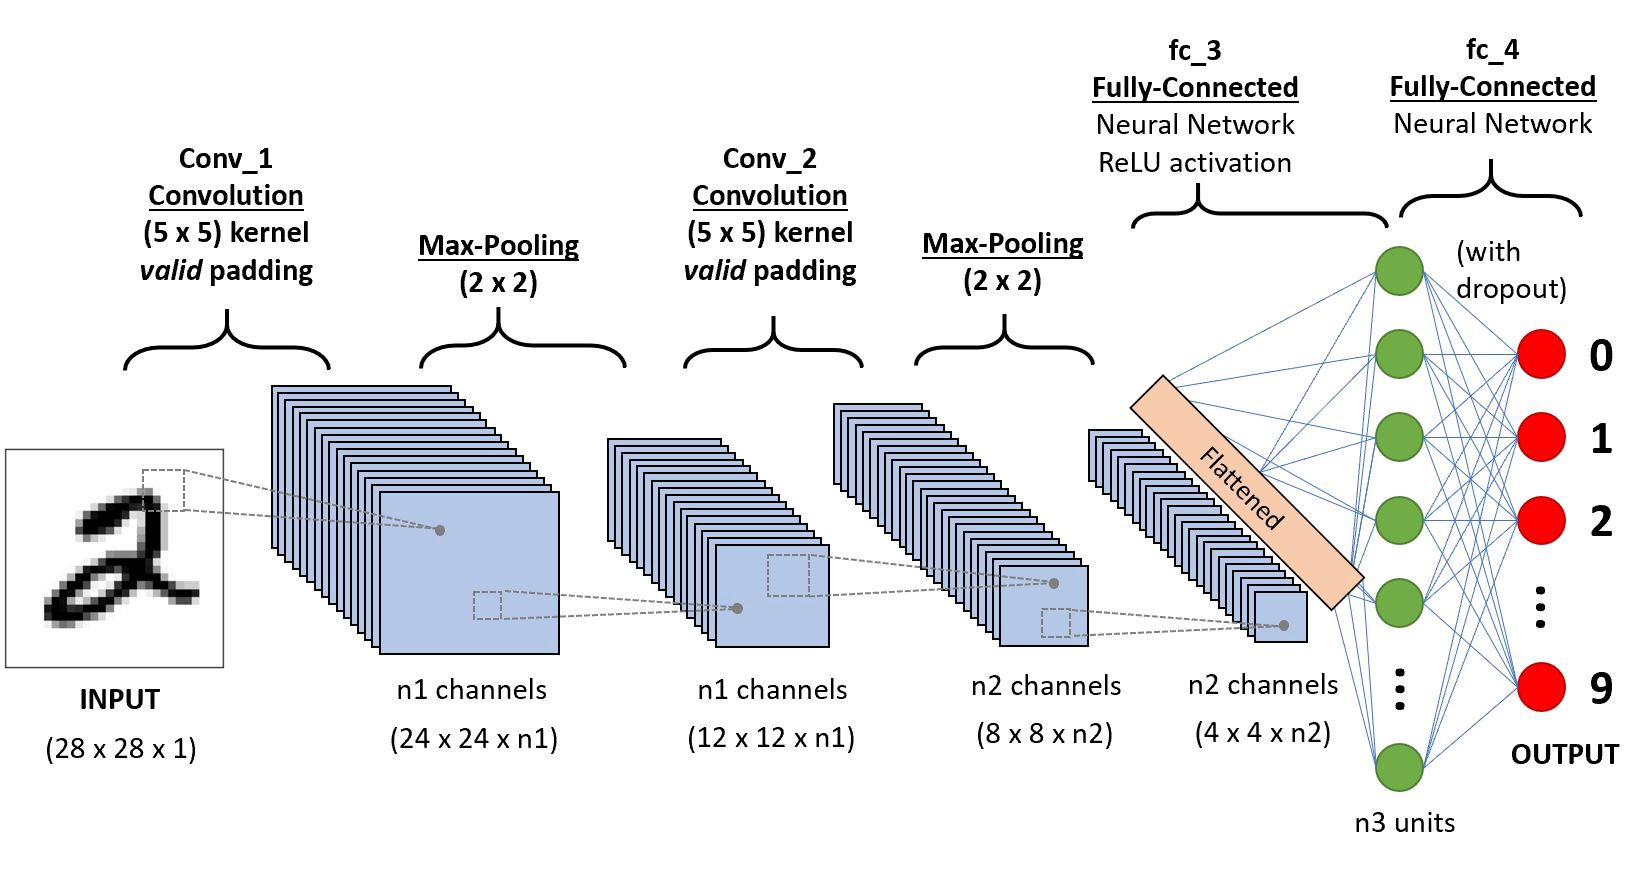
\includegraphics[width=0.9\linewidth]{cnn.jpeg}
  \caption{Convolutional neural network. \href{https://towardsdatascience.com/a-comprehensive-guide-to-convolutional-neural-networks-the-eli5-way-3bd2b1164a53}{Source}}
  \label{fig:cnn}
\end{figure}

\pagebreak\section{Applications}

Despite the difficulties associated with the development of computer vision, the considerable advances made over the years have already enabled Computer Vision to perform many tasks.

This technology is proving to be effective for optical character recognition, also known as "OCR", everyone with an Android smartphone can use it through Google Lens (see Figure ~\ref{fig:glens}).
\begin{figure}[H]
  \centering
  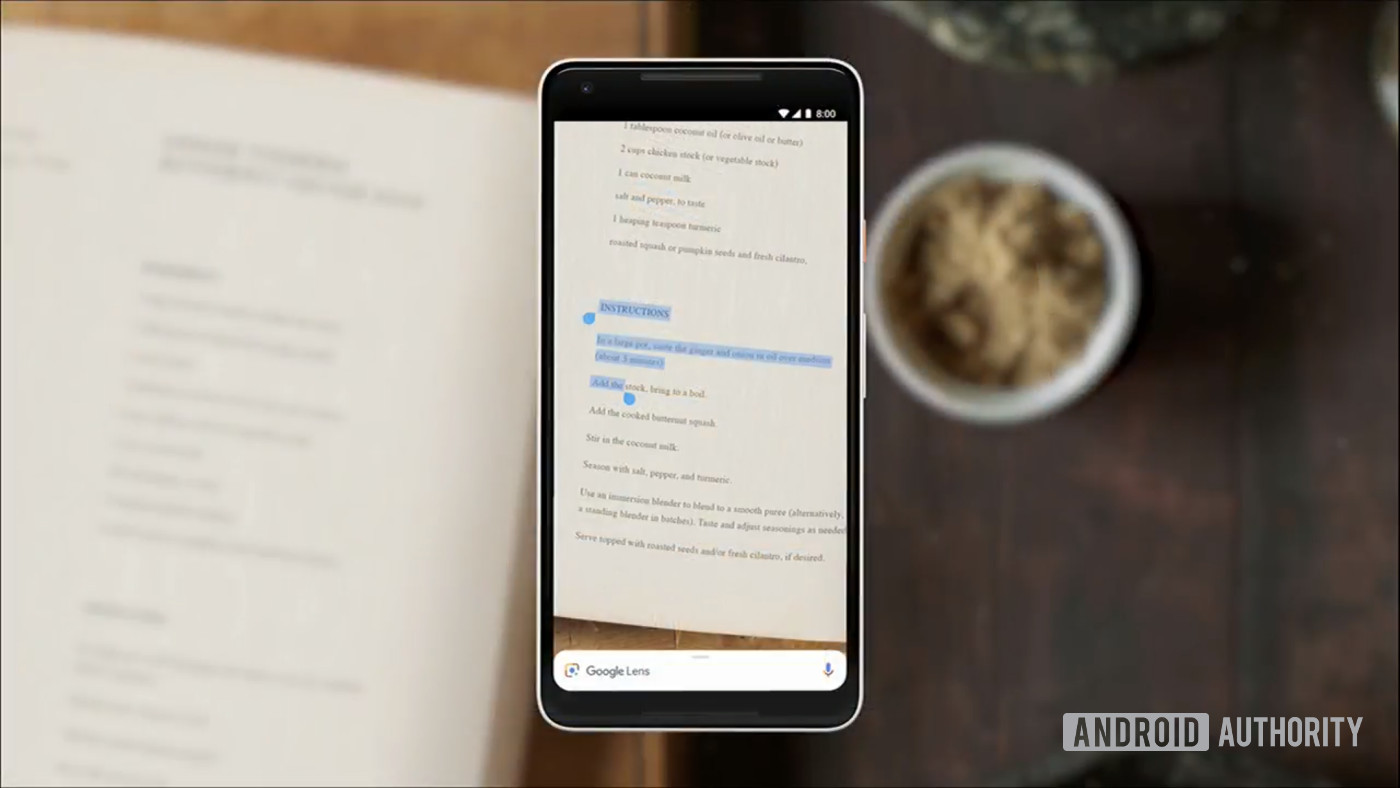
\includegraphics[width=.8\linewidth]{google-lens-smart-text-selection.jpg}
  \caption{Optical character recognition directly on your smartphone with Google Lens. \href{https://www.androidauthority.com/google-lens-camera-app-863117/}{Source}}
  \label{fig:glens}
\end{figure}
\pagebreak
In the field of automotive safety, computer vision is used for hazard detection. With the emergence of autonomous cars, computer vision will soon occupy a central place in the automotive industry as it will allow vehicles to see on the road (see an example of image segmentation in the field of smart vehicles on Figure ~\ref{fig:carseg}).

\begin{figure}[H]
  \centering
  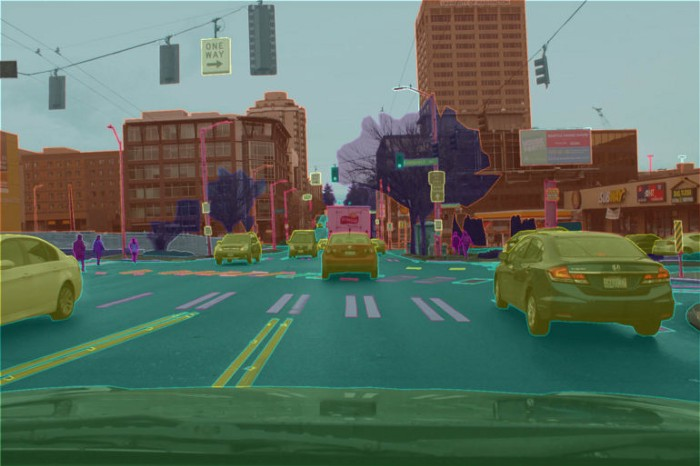
\includegraphics[width=.8\linewidth]{image_segmentation.jpg}
  \caption{Image segmentation on the road. \href{https://towardsdatascience.com/learning-computer-vision-41398ad9941f}{Source}}
  \label{fig:carseg}
\end{figure}%

\pagebreak
It is also used in the film industry for "match move", i.e. to synchronize computer-generated images with the real actors. It is also used for motion capture.

The facial recognition technologies of the latest smartphones, such as the famous Face ID of Apple's latest iPhone, are also based on Computer Vision. The same technology is used by automatic surveillance cameras (see face-related applications on Figure ~\ref{fig:facreco}).
\begin{figure}[H]
\centering
\begin{subfigure}{.5\textwidth}
  \centering
  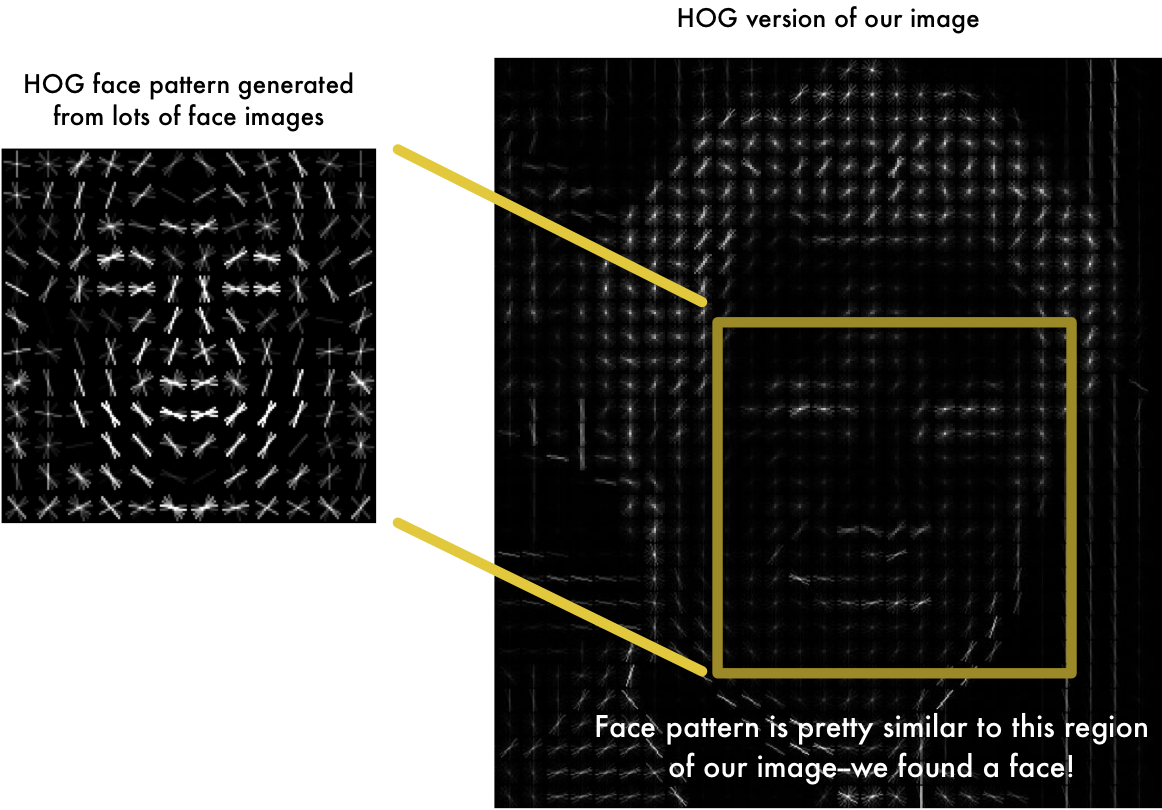
\includegraphics[width=.8\linewidth]{hog.png}
  \caption{Histogram of oriented gradients (used in facial recognition) \href{https://medium.com/@ageitgey/machine-learning-is-fun-part-4-modern-face-recognition-with-deep-learning-c3cffc121d78}{Source}}
\end{subfigure}%
\begin{subfigure}{.5\textwidth}
  \centering
  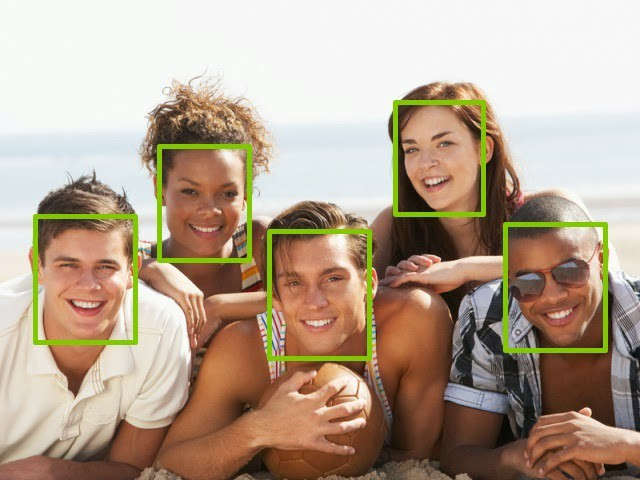
\includegraphics[width=.8\linewidth]{face_detection.jpg}
  \caption{Face detection. \href{https://towardsdatascience.com/learning-computer-vision-41398ad9941f}{Source}}
\end{subfigure}
\caption{Examples of face-related applications}
\label{fig:facreco}
\end{figure}

As you will have understood, computer vision is used in a wide range of fields. As this technology develops, the opportunities it offers will increase in the coming years. Soon, all machines will probably be able to see, in exactly the same way as human beings and better ...

Computer vision is not yet very practical to use on our current everyday interfaces: smartphones.
In the future, we can imagine increasing human vision by coupling it with computer vision via mixed reality glasses, for example looking at a monument, having its history displayed on the glasses...

\chapter{Related work}
\section{Object classification}
An example of object classification is whether, for a given image, if there is a cat or not in the image.

The most popular example of object classification is MNIST\cite{lecun-mnisthandwrittendigit-2010}, which was a task to find the number in the image (between 0 and 9).

Object classification is at the core of computer vision and it is probably the easiest task to solve.
This task could be used as an alternative to object detection though, because there isn't usually multiple animals anyway on the same picture and object classification is also faster since it doesn't have to infer location.

\pagebreak\subsection{Datasets}

\subsubsection{ImageNet}
ImageNet\cite{imagenet_cvpr09} is a database of annotated images produced by the organization of the same name for computer vision research. In 2016, more than ten million URLs were manually annotated to indicate which objects are represented in the image; more than one million images benefit in addition to bounding boxes around the objects. 
ImageNet is based on WordNet (see Figure ~\ref{fig:wordnet}) which is a semantic lexicon for the English language that is used extensively by computational linguists and cognitive scientists. Nouns, verbs, adjectives and adverbs are grouped into sets of cognitive synonym rings (synsets), each expressing a distinct concept. Synsets are interlinked by means of conceptual-semantic and lexical relations.
\begin{figure}[H]
  \centering
  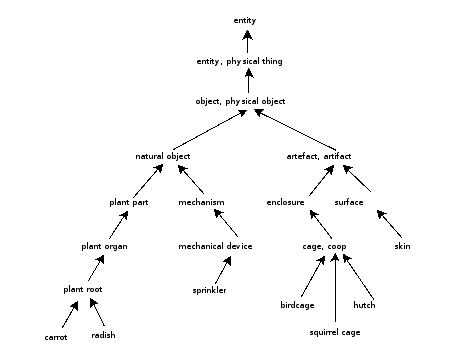
\includegraphics[width=.8\linewidth]{wordnet.png}
  \caption{WordNet directed acyclic graph. \href{http://www.cs.princeton.edu/courses/archive/spring07/cos226/assignments/wordnet.html}{Source}}
  \label{fig:wordnet}
\end{figure}
\pagebreak
The database of annotations on URLs of third-party images is freely available, but ImageNet does not own the images themselves. Since 2010, the ImageNet project has been organizing an annual competition: ImageNet Large Scale Visual Recognition Challenge (ILSVRC), or "ImageNet Large Scale Visual Recognition Competition". It consists of a software competition whose goal is to accurately detect and classify objects and scenes in natural images.

Imagenet is therefore a general classification dataset that aims to develop the vision in general, it is widely cited and widely used in many models

\pagebreak\subsection{Models}
\subsubsection{FixRes}
The top performance algorithm to date is called FixRes\cite{2019arXivFixRes}, it propose a simple but effective strategy to optimize classifier performance when train and test resolutions differ. It is only a fine adjustment of the network to the resolution of the test, inexpensive by calculation. This allows powerful classifiers to be trained using small training images. For example, FixRes achieve a top-1 accuracy of 77.1\% on ImageNet with a ResNet-50 trained on 128x128 images and 79.8\% with an image trained on 224x224 images.
Conversely, a pre-trained 32x48d ResNeXt-101 with low supervision on 940 million public images at 224x224 resolution and further optimizing the 320x320 test resolution, obtain a maximum accuracy of 86.4\% (top-5: 98.0)\%). 

FixRes is both a state of the art classification model on ImageNet\cite{pwc_classification_imagenet}, but also on iNaturalist\cite{pwc_classification_inaturalist}

\pagebreak\section{Object detection}
%https://medium.com/zylapp/review-of-deep-learning-algorithms-for-object-detection-c1f3d437b852
Object detection is locating instances of objects in images, for example, while you are looking at this text, you see multiple words next to each other, it is object detection.

Object detection models are more appropriate for identifying multiple relevant objects in a single image. The second important advantage of object detection models over image classification models is that the location of objects is provided.

\subsection{Datasets}
\subsubsection{COCO}
COCO\cite{coco} dataset is a collection of images of scenes of daily life containing common objects in their natural context (see Figure ~\ref{fig:coco}). Objects are labeled using instance-based segmentations to precise location of objects. The data set contains photos of 91 types of objects that are \begin{it}"easily recognizable by a 4-year-old child"\end{it}. With a 2.5 million instances tagged in 328,000 images.

COCO is widely used for object detection and image segmentation due to its recognition simplicity.

\begin{figure}[H]
    \centering
    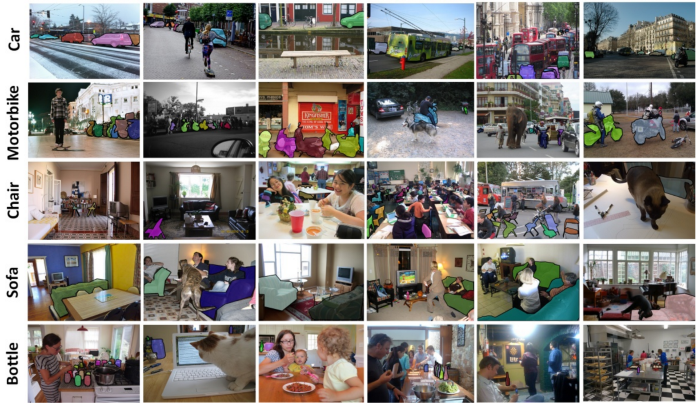
\includegraphics[scale = 0.6]{images/coco.png}
	\caption[Example COCO dataset]{Examples of segmented objects from the 2015 COCO dataset. \href{https://arxiv.org/pdf/1405.0312.pdf}{Source}}
	\label{fig:coco}
\end{figure}

\subsubsection{Open Image}
Open Image V4\cite{openimagev4} is a 9.2 million pixel image data set with unified annotations for image classification, object detection and visual relationship detection. The images have a Creative Commons Attribution license that allows you to share and adapt the material. They were collected from Flickr without a predefined list of class names or tags, thus generating natural class statistics and avoiding initial design bias. Open Images V4 offers a large scale in several dimensions: 30.1 million pixel image level labels for 19.8 KB concepts, 15.4 million pixel selection boxes for 600 object classes and 375,000 pixel visual relationship annotations for 57 classes. For object detection in particular, 15 times more enclosures is provided than the next largest datasets (15.4 million enclosures out of 1.9 million images). Images often show complex scenes with several objects (8 objects annotated per image on average). Visual relationships are annotated together, which support the detection of visual relationships, an emerging task that requires structured reasoning. Complete and detailed statistics on the dataset are provided, the quality of annotations are validated and the performance of many modern models evolution with increasing amounts of training data are delivered.

Open Image bring high quality images and is more complex for recognition than COCO, it also allow vision relationship detection.


\pagebreak\subsection{Models}
\subsubsection{Performance metrics}
\paragraph{Intersection on Union (IoU)}
IoU is a measure based on Jaccard Index that evaluates the overlap between two bounding boxes. It requires a ground truth bounding box \begin{math}B_{gt}\end{math} and a predicted bounding box \begin{math}B_{p}\end{math}. 
By applying the IoU we can tell if a detection is valid (True Positive) or not (False Positive).
IoU is given by the overlapping area between the predicted bounding box and the ground truth bounding box divided by the area of union between them: 
\begin{gather*}
\centering
\mathrm{IoU}=\frac{\operatorname{area}\left(B_{p} \cap B_{g t}\right)}{\operatorname{area}\left(B_{p} \cup B_{g t}\right)}
\end{gather*}

IoU is a value between 0 and 1, which corresponds to the overlap zone between the predicted zone and the truth zone on the ground. The higher the IoU value, the better the intended location of the box for a given object. Usually, we keep all candidates in the bounding box with an IoU above a threshold.

\pagebreak\paragraph{mean Average Precision (mAP)}

A common metric which is used for the Pascal VOC object recognition challenge is to measure the Average Precision (AP) for each class. The following description of Average Precision is taken from Everingham et. al.\footnote{\href{http://homepages.inf.ed.ac.uk/ckiw/postscript/ijcv_voc09.pdf}{Source}}

\begin{it}
The mean Average Precision (mAP) is computed by taking the average over the APs of all classes.
For a given task and class, the precision/recall curve is computed from a method’s ranked output. Recall is defined as the proportion of all positive examples ranked above a given rank. Precision is the proportion of all examples above that rank which are from the positive class. The AP summarizes the shape of the precision/recall curve, and is defined as the mean precision at a set of eleven equally spaced recall levels [0,0.1, . . . ,1]:
\begin{gather*}
    A P=\frac{1}{11} \sum_{r \in\{0,0,1, \ldots, 1\}} p_{i n t e r p}(r)
\end{gather*}

The precision at each recall level r is interpolated by taking the maximum precision measured for a method for which the corresponding recall exceeds r:
\begin{gather*}
    p_{\text {interp}}(r)=\max _{\tilde{r} : \tilde{r} \geq r} p(\tilde{r})
\end{gather*}

where p(˜r) is the measured precision at recall ˜r. The intention in interpolating the precision/recall curve in this way is to reduce the impact of the “wiggles” in the precision/recall curve, caused by small variations in the ranking of examples. It should be noted that to obtain a high score, a method must have precision at all levels of recall – this penalizes methods which retrieve only a subset of examples with high precision (e.g. side views of cars).
\end{it}



\pagebreak\subsubsection{Convolutional network based on the region (R-CNN)}
The region-based convolutional network is one of the main contemporary approach to object detection,
In R-CNN\cite{rcnn}, a selective search algorithm was used. Selective search is one of the generic object proposal generation methods.
\begin{enumerate}
    \item Try to detect objects
    \item Run a CNN on these objects
    \item Run the output into a SVM to classify the object and a linear regressor to adjust the box
\end{enumerate}
This approach can be expensive however because many crops are necessary, leading to significant duplicated computation from overlapping crops (see Figure ~\ref{fig:rcnn}).

\begin{figure}[H]
    \centering
    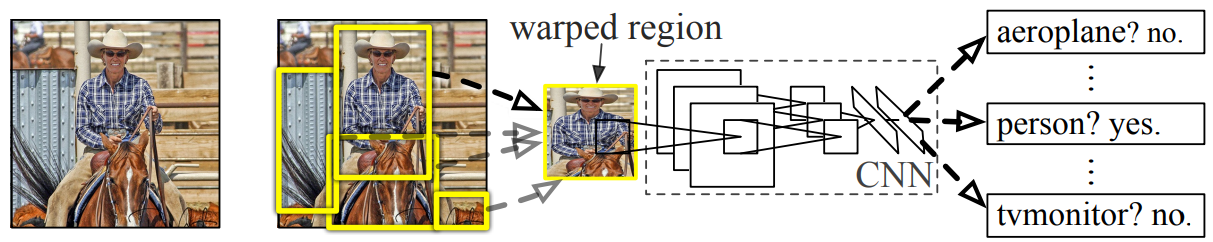
\includegraphics[scale = 0.35]{rcnn.png}
	\caption[R-CNN]{Region-based Convolution Network. (R-CNN). \href{https://arxiv.org/pdf/1311.2524v5.pdf}{Source}}
	\label{fig:rcnn}
\end{figure}


\pagebreak\subsubsection{Convolutional network based on a fast region (Fast R-CNN)}
The convolutional network based on the fast region (Fast R-CNN)\cite{fastrcnn} aims to reduce the time consumption related to the large number of models required to analyze all region proposals (see Figure ~\ref{fig:fastrcnn}).
\begin{enumerate}
    \item Performing feature extraction before proposing regions, therefore only running one CNN over the entire image instead of a CNN CNN per region
    \item Replacing the SVM with a softmax layer, therefore extending the neural network for predictions instead of creating a new model
\end{enumerate}

\begin{figure}[H]
    \centering
    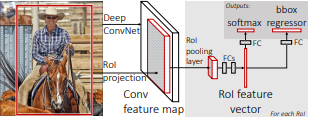
\includegraphics[scale = 0.8]{fast_rcnn.png}
	\caption[Fast R-CNN]{Region-based Convolution Network. (R-CNN). \href{https://arxiv.org/pdf/1504.08083.pdf}{Source}}
	\label{fig:fastrcnn}
\end{figure}

\pagebreak\subsubsection{Convolutional network based on faster regions (Faster R-CNN)}
The region proposals detected with the selective search method were still needed in the previous model, which is expensive in terms of calculation. 

Faster R-CNN\cite{fastrcnn} introduced the Regional Proposal Network (RPN) (see Figure ~\ref{fig:rpn}) to directly generate regional proposals, predict selection frameworks and detect objects. The convolutional network based on a faster region (Faster R-CNN) is a combination of the RPN model and the Fast R-CNN model.

\begin{enumerate}
    \item At the last layer of an initial CNN, a 3x3 sliding window moves across the feature map and maps it to a lower dimension (256-d)
    \item For each sliding-window location, it generates multiple possible regions based on k fixed-ratio anchor boxes
    \item Each region proposal consists of an “objectness” score for that region and 4 coordinates representing the bounding box of the region
\end{enumerate}


\begin{figure}[H]
    \centering
    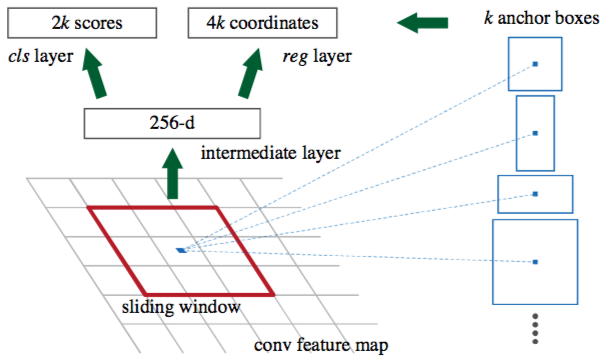
\includegraphics[scale = 0.5]{faster_rcnn.png}
	\caption[Region Proposal Network]{Region Proposal Network.  \href{https://arxiv.org/pdf/1506.01497.pdf}{Source}}
	\label{fig:rpn}
\end{figure}

The faster R-CNN uses RPN to avoid the selective search method, it speeds up training and testing processes and improves performance.

\begin{comment} % add or not
\begin{figure}[H]
    \centering
    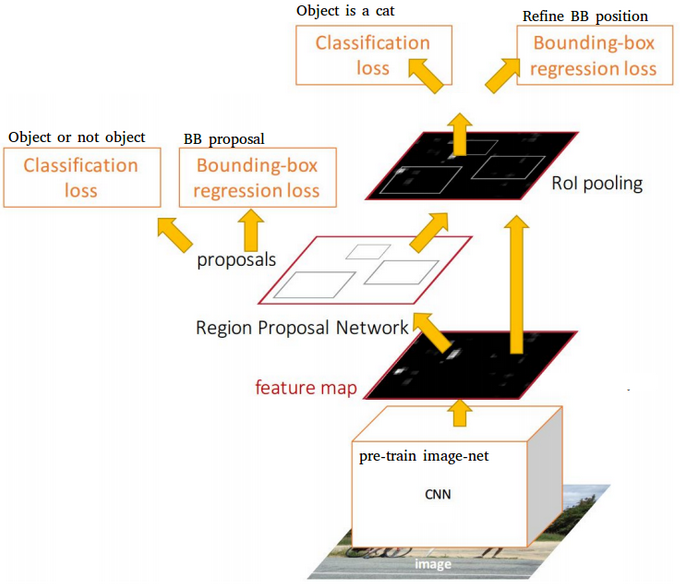
\includegraphics[scale = 0.35]{faster_rcnn2.png}
	\caption[Faster R-CNN]{Faster R-CNN = RPN + Fast R-CNN.   \href{https://arxiv.org/pdf/1506.01497.pdf}{Source}}
\end{figure}
\end{comment}


\pagebreak\subsubsection{Fully convolutional region-based network (R-FCN)}
The fast and rapid methodologies of R-CNN consist in detecting region proposals and recognizing an object in each region. The fully convolutional region-based network (R-FCN) is a model with only convolutional layers allowing to share all the computation.

R-FCN merge the two basic steps into a single model to simultaneously take into account object detection (location invariant) and its position (location variant).

\begin{enumerate}
    \item Run a CNN over the input image
    \item Add a fully convolutional layer to generate a score bank of the aforementioned “position-sensitive score maps.” There should be k²(C+1) score maps, with k² representing the number of relative positions to divide an object (e.g. 3² for a 3 by 3 grid) and C+1 representing the number of classes plus the background.
    \item Run a fully convolutional region proposal network (RPN) to generate regions of interest (RoI’s)
    \item For each RoI, divide it into sub-regions as the score maps
    \item For each sub-regions, compare with the score bank to see if it matches the corresponding position of some object.
    \item Once each of the sub-regions has an object match value for each class, average the sub-regions to get a single score per class.
    \item Classify the RoI with a softmax over the remaining C+1 dimensional vector
\end{enumerate}


\begin{figure}[H]
    \centering
    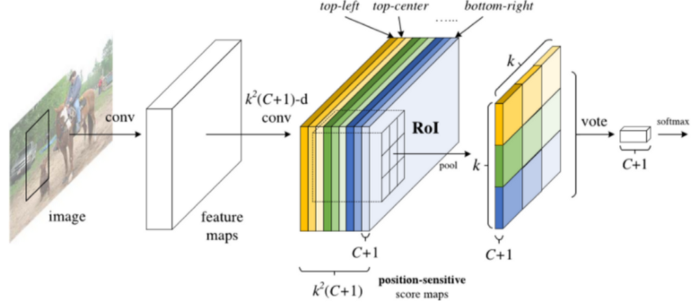
\includegraphics[scale = 0.5]{rfcn.png}
	\caption[R-FCN]{Fully convolutional region-based network. \href{https://arxiv.org/pdf/1605.06409.pdf}{Source}}
\end{figure}

In simple terms, the R-FCN examines each region proposal, dividing it into sub-regions.
For each sub-region, he asks: "Does it look like the left end of a baby?", "Does it look like the upper center of a baby?" "Does it look like a baby's top right?" etc. For all possible classes.  If enough sub-regions say "yes, I match up with a part of a baby", the RoI is classified as a baby after a softmax over all classes (see Figure ~\ref{fig:rfcnbaby}).


\begin{figure}[H]
    \centering
    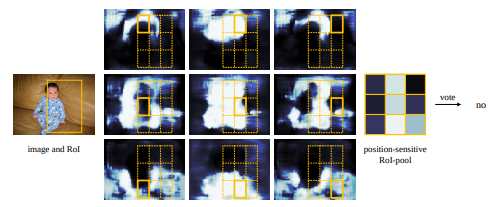
\includegraphics[scale = 0.7]{rfcn2.png}
	\caption[R-FCN2]{Visualization of R-FCN (k × k = 3 × 3) for the person category.  \href{https://arxiv.org/pdf/1605.06409.pdf}{Source}}
	\label{fig:rfcnbaby}
\end{figure}

\begin{figure}[H]
    \centering
    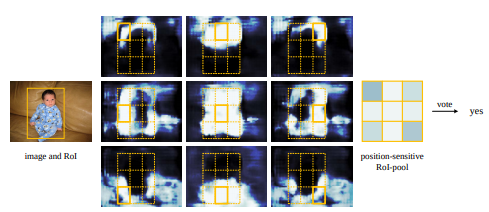
\includegraphics[scale = 0.7]{rfcn3.png}
	\caption[R-FCN3]{Visualization when an RoI does not correctly overlap the object.  \href{https://arxiv.org/pdf/1605.06409.pdf}{Source}}
\end{figure}



\pagebreak\subsubsection{You only look once (YOLO)}
The YOLO\cite{yolo} model directly predicts bounding boxes and class probabilities with a single network in a single assessment. The simplicity of the YOLO model allows real-time predictions.
YOLO is doing an end-to-end learning paradigm: proposals, features, and the classifier becoming one neural network (see Figure ~\ref{fig:yolo}). 

One indispensable component is non-maximum suppression (NMS), a post-processing algorithm responsible for merging all detections that belong to the same object. 

\begin{enumerate}
    \item Split our image into cells. Each cell will be responsible for predicting bounding boxes score, this score is simply the probability to detect the object multiplied by the IoU between the predicted and the ground truth boxes.
    \item Remove boxes with low object probability and bounding boxes with the highest shared area in the process called non-max suppression.
\end{enumerate}


\begin{figure}[H]
    \centering
    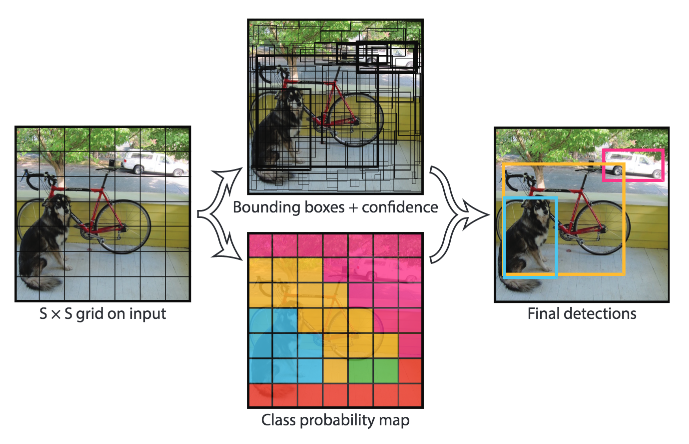
\includegraphics[scale = 0.5]{yolo.png}
	\caption[YOLO]{Imaged example of the steps of YOLO. \href{https://arxiv.org/pdf/1506.02640.pdf}{Source}}
	\label{fig:yolo}
\end{figure}

\begin{comment}
\begin{figure}[H]
    \centering
    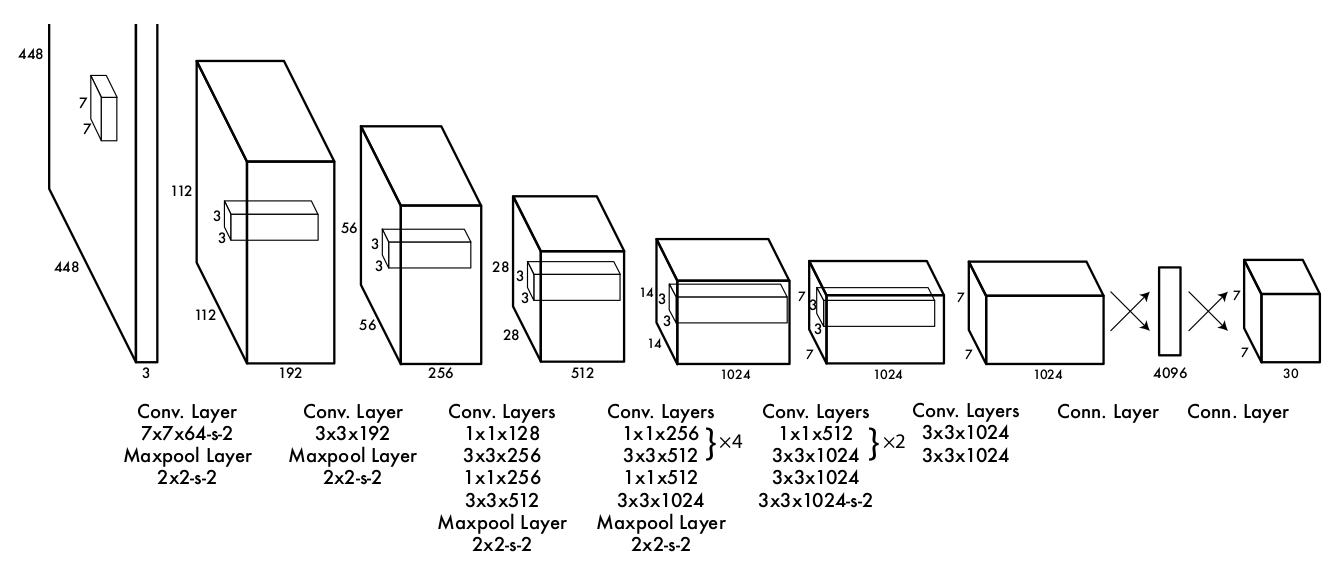
\includegraphics[scale = 0.20]{yolo2.png}
	\caption[YOLO2]{YOLO architecture \href{https://arxiv.org/pdf/1506.02640.pdf}{Source}}
\end{figure}
\end{comment}


\pagebreak\subsubsection{Single-shot detector (SSD)}
Similar to the YOLO model, Single Shot Detector (SSD)\cite{ssd} predict both bounding boxes and class probabilities with an end-to-end CNN architecture (see Figure ~\ref{fig:ssdyolo}).

The SSD model uses extra feature layers from different feature maps of the network in order to increase the number of relevant bounding boxes.

\begin{enumerate}
    \item The model takes as input an image that passes through several convolution layers with different filter sizes (10x10, 5x5 and 3x3) that will generate feature maps.
    \item Each location in these feature maps are processed by specific convolution layers with 3x3 filters, to produce a set of bounding boxes similar to the Fast R-CNN anchor boxes.
    \item For each box, simultaneously predict the bounding box location and the class probabilities.
    \item During training, match the ground truth box with these predicted boxes based on IoU. The best predicted box will be labeled a “positive,” along with all other boxes that have an IoU with the truth > 0.5.
\end{enumerate}



\begin{figure}[H]
    \centering
    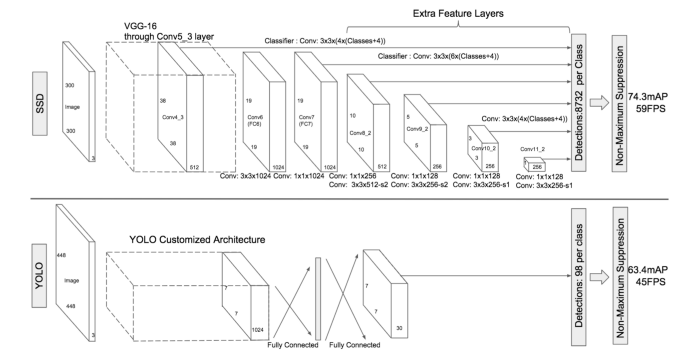
\includegraphics[scale = 0.5]{ssd.png}
	\caption[SSD]{Comparison between the SSD and the YOLO architectures. \href{https://arxiv.org/pdf/1512.02325.pdf}{Source}}
	\label{fig:ssdyolo}
\end{figure}
\pagebreak
The varying-size feature maps brought by SSD help capture objects of different sizes. Here is an example of SSD inference (see Figure ~\ref{fig:ssdinf}).

\begin{figure}[H]
    \centering
    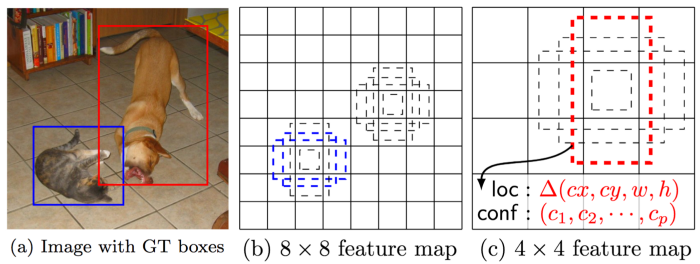
\includegraphics[scale = 0.5]{ssd2.png}
	\caption[SSD2]{SSD Framework. \href{https://arxiv.org/pdf/1512.02325.pdf}{Source}}
	\label{fig:ssdinf}
\end{figure}

In the end SSD does two things:
\begin{itemize}
    \item First, apply non-maximum suppression to group boxes that overlap strongly. In other words, if four boxes of similar shapes, sizes, etc. contain the same cat, NMS will keep the one with the most confidence and reject the rest. 
    \item Second, the model uses a technique called hard negative mining to balance classes during training. In the case of hard negative mining, only a subset of the negative examples with the highest training loss (i.e. false positives) are used for each iteration of the training. SSD maintains a 3:1 ratio between negatives and positives.
\end{itemize}

\pagebreak\subsubsection{Neural Architecture Research Network (NASNet)}

NASNet\cite{nasnet} consists in learning the architecture of a model using reinforcement learning to optimize the number of layers while improving the accuracy of a given data set. NASNet achieved superior performance with a lighter model than previous work compared to the 2012 ImageNet classification challenge (see Figure ~\ref{fig:nasnet}).
The NASNet network has an architecture learned from the CIFAR-10\cite{cifar10} dataset and is trained in the ImageNet 2012 dataset.

From the official paper:

\begin{it}
"Our approach is inspired by the recently proposed Neural Architecture Search (NAS) framework, which uses a reinforcement learning search method to optimize architecture configurations. Applying NAS, or any other search methods, directly to a large dataset, such as the ImageNet dataset, is however computationally expensive. We therefore propose to search for a good architecture on a proxy dataset, for example the smaller CIFAR-10 dataset, and then transfer the learned architecture to ImageNet."
\end{it}

\begin{figure}[H]
    \centering
    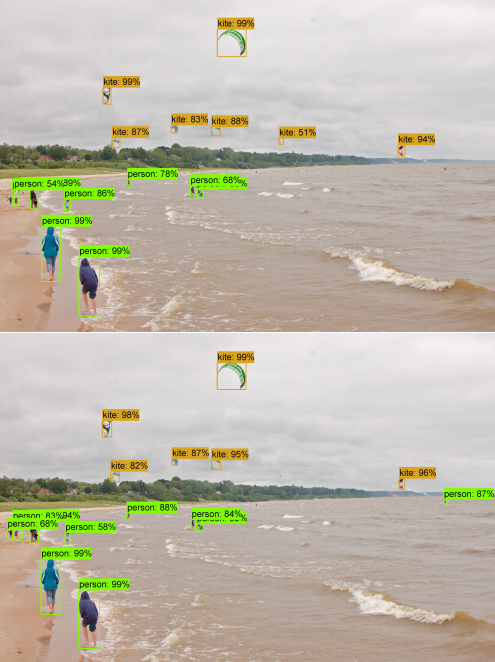
\includegraphics[scale = 0.4]{nasnet.png}
	\caption[NASNet]{Example of object detection results differences between Faster-RCNN
    with Inception-ResNet-v2 featurization (top) and NASNet-A featurization (bottom). \href{https://arxiv.org/pdf/1707.07012.pdf}{Source}}
    \label{fig:nasnet}
\end{figure}

\pagebreak\subsubsection{Convolutional network based on a mask region (Mask R-CNN)}
Mask R-CNN\cite{maskrcnn} is an extension over Faster R-CNN. Faster R-CNN predicts bounding boxes and Mask R-CNN essentially adds one more branch for predicting an object mask in parallel (see example on Figure ~\ref{fig:maskrcnn}).

\begin{figure}[H]
    \centering
    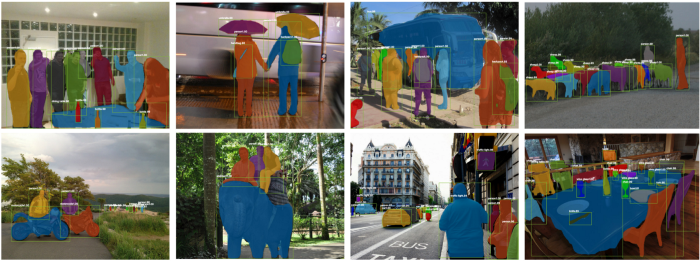
\includegraphics[scale = 0.5]{mask_rcnn.png}
	\caption[Mask R-CNN2]{Examples of Mask R-CNN application on the COCO test dataset.  \href{https://arxiv.org/pdf/1703.06870.pdf}{Source}}
	\label{fig:maskrcnn}
\end{figure}

There are two stages of Mask R-CNN (see Figure ~\ref{fig:maskrcnn2}). 
\begin{enumerate}
    \item Generates proposals about the regions where there might be an object based on the input image.
    \item Predicts the class of the object, refines the bounding box and generates a mask in pixel level of the object based on the first stage proposal. Both stages are connected to the backbone structure.
\end{enumerate}

\begin{it}
"The mask branch is a small FCN applied to each RoI, predicting a segmentation mask in a pixel-to-pixel manner."\cite{maskrcnn}
\end{it}

\begin{figure}[H]
    \centering
    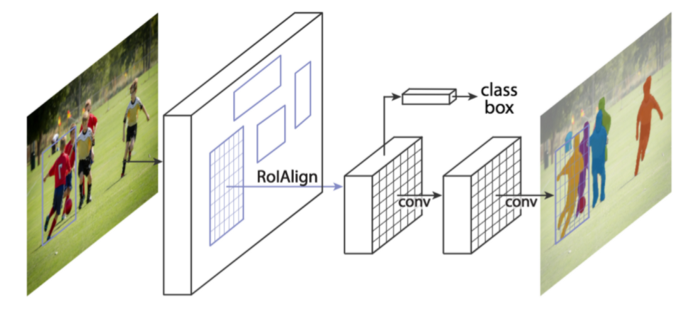
\includegraphics[scale = 0.5]{mask_rcnn2.png}
	\caption[Mask R-CNN2]{Mask R-CNN framework for instance segmentation. \href{https://arxiv.org/pdf/1703.06870.pdf}{Source}}
	\label{fig:maskrcnn2}
\end{figure}

\pagebreak\subsection{Object detection conclusion}
Over the years, object detection models tend to infer that location and classification have a fully differentiable network. Therefore, it can be trained from head to tail with neural networks in a end-to-end manner.

The most important question is not which detector is the best. It may not be possible to answer. The real question is which detector and which configurations offer us the best balance between speed and accuracy that your application needed. Below is a comparison of the accuracy vs speed tradeoff (time measured in milliseconds) (see Figure ~\ref{fig:odbenchmark}).

\begin{figure}[H]
    \centering
    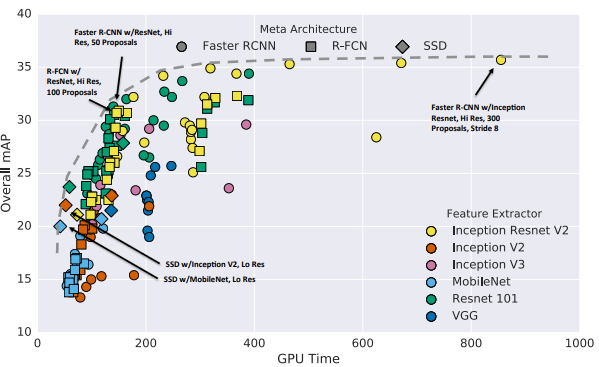
\includegraphics[scale = 0.7]{object_detection_benchmark.png}
	\caption{Object detection speed vs accuracy tradeoff. \href{https://arxiv.org/pdf/1611.10012.pdf}{Source}}
	\label{fig:odbenchmark}
\end{figure}

\pagebreak\section{Action classification}

Learning to understand videos is a very difficult task, both in terms of algorithms and calculations, the networks have access to not only the appearance information present in single, static images, but also their complex temporal evolution. 
Such a task could be useful to analyse wildlife behaviours, a kind of information that is very rare.

\subsection{Datasets}

\subsubsection{Charades}
Charades-Ego\cite{charades} is a 68,536 instances of activity in 68.8 hours of first and third person video, making it one of the largest and most diverse egocentric data sets in the world. Charades-Ego also shares activity classes, scripts and methodology with the Charades data set, which consists of an additional 82.3 hours of third person video with 66,500 activity instances. Charades-Ego has time annotations and text descriptions, making it suitable for self-centered video classification, localization, subtitling and new tasks using the inter-modal nature of data.

\subsubsection{Moments in Time}
Moments in Time\cite{momentsintime} dataset is a large-scale collection of one million short videos, annotated by man, corresponding to dynamic events taking place in less than three seconds. Modelling spatio-temporal dynamics, even for actions made in 3-second videos, poses many challenges: significant events include not only people, but also objects, animals and natural phenomena; visual and auditory events can be time-symmetric ("opening" is "closing" in the opposite direction) and transient or prolonged. The annotation process (each video is labelled with an action or activity label among 339 different classes), analyze its scale and diversity compared to other large-scale video data sets for action recognition, and present the results of several basic models. treat separately and jointly three modalities: spatial, temporal and auditory. The Moments in Time dataset, designed to cover many visual and auditory events and a wide variety of events, can be a new challenge in developing models that adapt to the level of complexity and abstract reasoning that a human deals with on a daily basis.

\pagebreak\subsection{Models}
\subsubsection{AssembleNet}
Standard CNN video CNN architectures have been designed by directly extending architectures designed for image understanding to a third dimension (using a limited number of spatio-temporal modules such as 3D convolutions) or by introducing a handmade two-stream design to capture both appearance and motion in videos. AssembleNet\cite{assemblenet} interpret a video CNN as a collection of multi-flow space-time convolution blocks connected to each other, and propose the approach of automatically searching for neural architectures with better connectivity for video comprehension. This is done by developing a population of overly connected architectures guided by learning the connection weight. Architectures combining representations that do not have different types of input (i.e. RGB and optical flow) at multiple temporal resolutions are sought, thus allowing different types or sources of information to interact. AssembleNet, surpasses previous approaches to public video data sets, in some cases with a large margin.

\pagebreak\section{Visual object tracking}

Visual object tracking is an interesting task that could also help to understand the species behaviour, for example if you can see on large amount of data that certain animal often goes into a certain direction ...

\subsection{Datasets}
\subsubsection{VOT}
The VOT2018\cite{vot2018} Challenge, followed by visual objects, is the sixth annual comparative analysis of monitoring organized by the VOT initiative. The results of more than 80 trackers are presented; many are leading trackers published at major computer vision conferences or in journals in recent years. The evaluation included the standard VOT method and other popular short-term follow-up analysis methods and a "real time" experiment simulating a situation in which a tracker treats images as if they were provided by a continuously operating sensor. A long-term monitoring sub-challenge has been introduced for all standard VOT sub-challenges. The new sub-challenge addresses the long-term monitoring properties, namely the management of target disappearance and reappearance. A new data set has been compiled and a performance evaluation methodology focusing on long-term monitoring capacities has been adopted. The VOT toolbox has been updated to support standard and long-term short-term monitoring sub-challenges. The performance of the follow-ups tested generally far exceeds the standard reference levels.

\pagebreak\subsection{Models}
\subsubsection{THOR}
Currently, the state-of-the-art algorithm to date on the VOT challenge is called thor\cite{thor}:

This algorithm focus on the construction of holistic object representations for tracking. The structure exploits the idea of obtaining additional object models during the tracking process. The resulting representation contains information beyond the location of the truth object on the ground provided to the system. It is then useful for orientation, but also for other tasks requiring a visual understanding of objects. Strong empirical results on monitoring benchmarks indicate that the method can improve the performance and robustness of underlying monitoring while reducing its speed. In addition, the method is able to reproduce current results, while using a simpler and older network architecture and operating three times faster.


\pagebreak\section{Wild life}

During the past decades, engineers and wildlife researchers have developed various hardware technologies for professionals to monitor individual mammals,
including very high frequency (VHF) radio tracking\cite{radio1983}\cite{inradio}\cite{satellite2018}, 
and Global Positioning System (GPS) tracking \cite{zebranet2002}\cite{gps2001}\cite{kruger2016inexpensive},
wireless sensor networks\cite{sensornet2002}\cite{sensornet2004},  
animal-mounted video monitoring systems \cite{portablecamera2008}, 
drones to captures images from above\cite{s16010097} and ultimately motion-triggered cameras which are useful to capture images only when an animal is present and in his natural environment including at night thanks to infrared.


A motion-triggered camera is a camera with an automatic gesture detection system, which activates the shot as soon as the sensor detects a movement (see example on Figure ~\ref{fig:camtrap}). 
Its continuous image analysis operation is similar to the proximity sensor with the additional capabilities to be transported, adapt to a medium, record and process images.

\begin{figure}[H]
\centering
\begin{subfigure}{.5\textwidth}
  \centering
  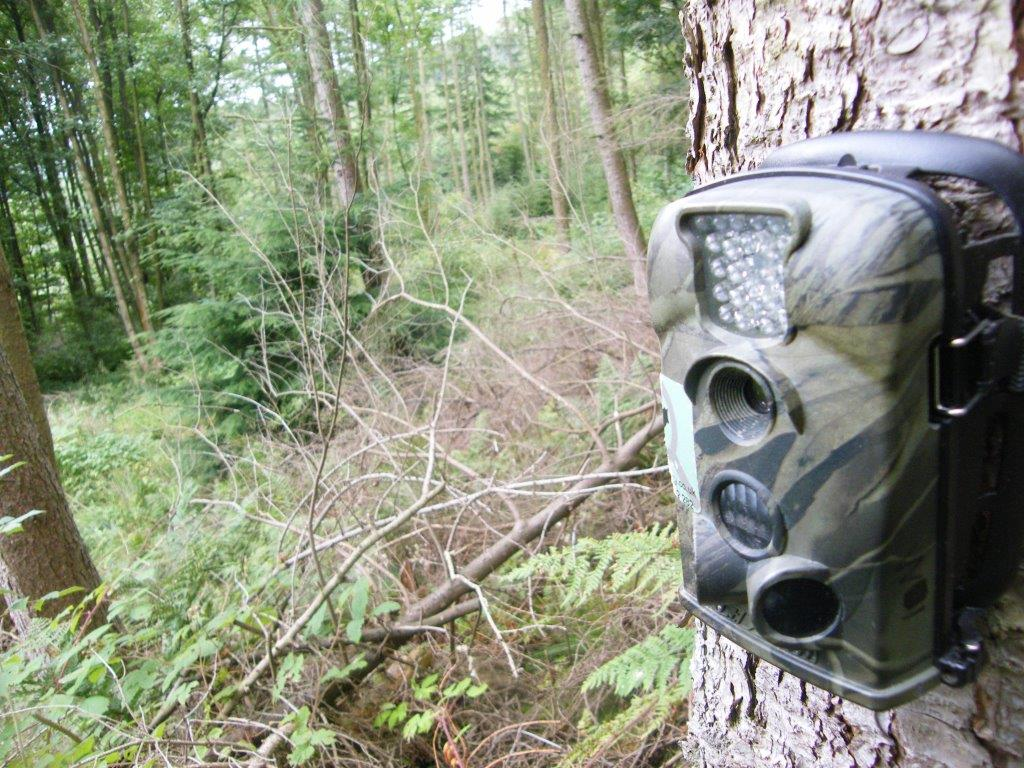
\includegraphics[width=.8\linewidth]{camera_trap.jpg}
  \caption{Camera trap. \href{https://shop.naturespy.org/wp-content/uploads/2014/05/Ltl-Acorn-camera-trap-1.jpg}{Source}}
\end{subfigure}%
\begin{subfigure}{.5\textwidth}
  \centering
  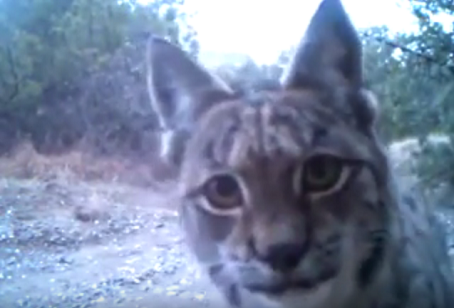
\includegraphics[width=.8\linewidth]{lynx.png}
  \caption{Lynx taken by camera trap. \href{https://agenda.ge/en/news/2015/2337}{Source}}
\end{subfigure}
\caption{Camera trap \& Picture taken by it}
\label{fig:camtrap}
\end{figure}

\pagebreak\subsection{Datasets}

\subsubsection{iNaturalist}
iNaturalist is a citizen science project and an online social network of naturalists, citizen scientists and biologists based on the concept of mapping and sharing biodiversity observations around the world. iNaturalist is accessible through its website or mobile applications. Observations recorded with iNaturalist provide valuable open data for scientific research projects, conservation agencies, other organizations and the public. The project has been described as "flagship for mobile natural history applications.
The dataset consists of 859,000 images from over 5,000 different species of plants and animals.
iNaturalist is different from camera trap datasets, it is probably between camera trap and ImageNet-like dataset since it is taken by amateurs.

\subsubsection{iWildCam 2018 Challenge Dataset}
iWildCam\cite{iwildcam2019} consists of 292,732 images on 143 locations in American SouthWest, each labelled either as containing an animal or as empty.

iWildCam is also a challenge in which training data and test data come from different regions. The species observed in each region overlap, but are not identical.

iWildCam 2018 is the biggest public camera-trap dataset for southwest wildlife.

\subsubsection{North American Camera Trap Images}
This data set\cite{north_american_camera_trap_and_resnet18} contains 3.7 million photographic trap images from five different locations in the United States, with tags for 28 animal categories, mainly at the species level (for example, the most common tags are cattle, boars and deer). About 12\% of the images are labelled as empty.
North American Camera Trap Images is the biggest public camera-trap dataset for north American wildlife


\pagebreak\subsubsection{Snapshot Seregenti}
Hundreds of camera traps in Tanzania's Serengeti National Park open a powerful new window into the dynamics of Africa's most elusive wildlife species. The camera traps have been in continuous operation since 2010 and has produced millions of images, classified by volunteers.

This data set contains approximately 2.5 million camera trap image sequences, for a total of 6.7 million images, from seasons one to ten of the Snapshot Serengeti project. Tags are provided for 55 animal categories, mainly at the species level (for example, the most common tags are wildebeest, zebra and Thomson's gazelle). About 75\% of the images are labelled as empty. There is approximately 150,000 selection box annotations to approximately 78,000 of these images.

Snapshot Seregenti is surely the biggest public camera-trap dataset for African wildlife.

\pagebreak\subsubsection{Synthetic data}
Synthetic data and simulated environment are really promising, the advances in the field of computer graphics enable the modeling of 3D world looking closely to reality and can be generated infinitely.
Airsim\cite{airsim} is an open source system designed to form autonomous systems. AirSim provides realistic environments, vehicle dynamics and multimodal detection to researchers who build autonomous vehicles using AI to improve their safe operation in an open world.

Engineers who build autonomous systems can create accurate and detailed models of systems and environments, making them intelligent using methods such as in-depth learning, imitation learning and reinforcement learning. Tools such as Bonsai can be used to train models for a variety of environmental conditions and vehicle scenarios in the cloud on Microsoft Azure - much faster and safer than what is feasible in the real world. Once the training is complete, designers can deploy these trained models on real hardware.
Airsim has evolved towards a general purpose simulated environment and now contains also wildlife and camera-traps (see Figure ~\ref{fig:airsim}).

\begin{figure}[H]
\centering
\begin{subfigure}{.5\textwidth}
  \centering
  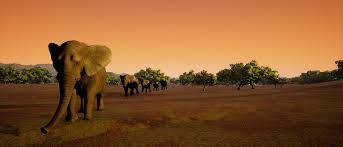
\includegraphics[width=.8\linewidth]{airsim_elephant.jpeg}
  \caption{Airsim elephant. \href{http://teamcore.usc.edu/papers/2018/bondi_camera_ready_airsim-w.pdf}{Source}}
\end{subfigure}%
\begin{subfigure}{.5\textwidth}
  \centering
  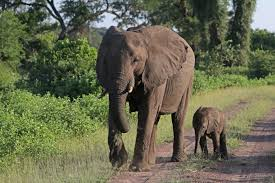
\includegraphics[width=.8\linewidth]{real_elephant.jpeg}
  \caption{Real elephant. \href{https://commons.wikimedia.org/wiki/User:Charlesjsharp/favourites}{Source}}
\end{subfigure}
\caption{Example showing differences between synthetic and real animal}
\label{fig:airsim}
\end{figure}

Synthetic data are still far from real data but it can still be used to learn the general pattern of specific data, the advantage is that synthetic data are unlimited.

\pagebreak\subsection{Models}

In the case of camera-trap images, we can't simply directly use the same models that has been trained on animal images taken by professionals.
Motion triggered camera images have lower quality and are highly cluttered with low contrast, and with dramatic background motion. Pattern detection also needs to handle a wide variety of animal body sizes, appearance, and poses (see differences example in Figure ~\ref{fig:camtraprealcam}).

\begin{figure}[H]
\centering
\begin{subfigure}{.5\textwidth}
  \centering
  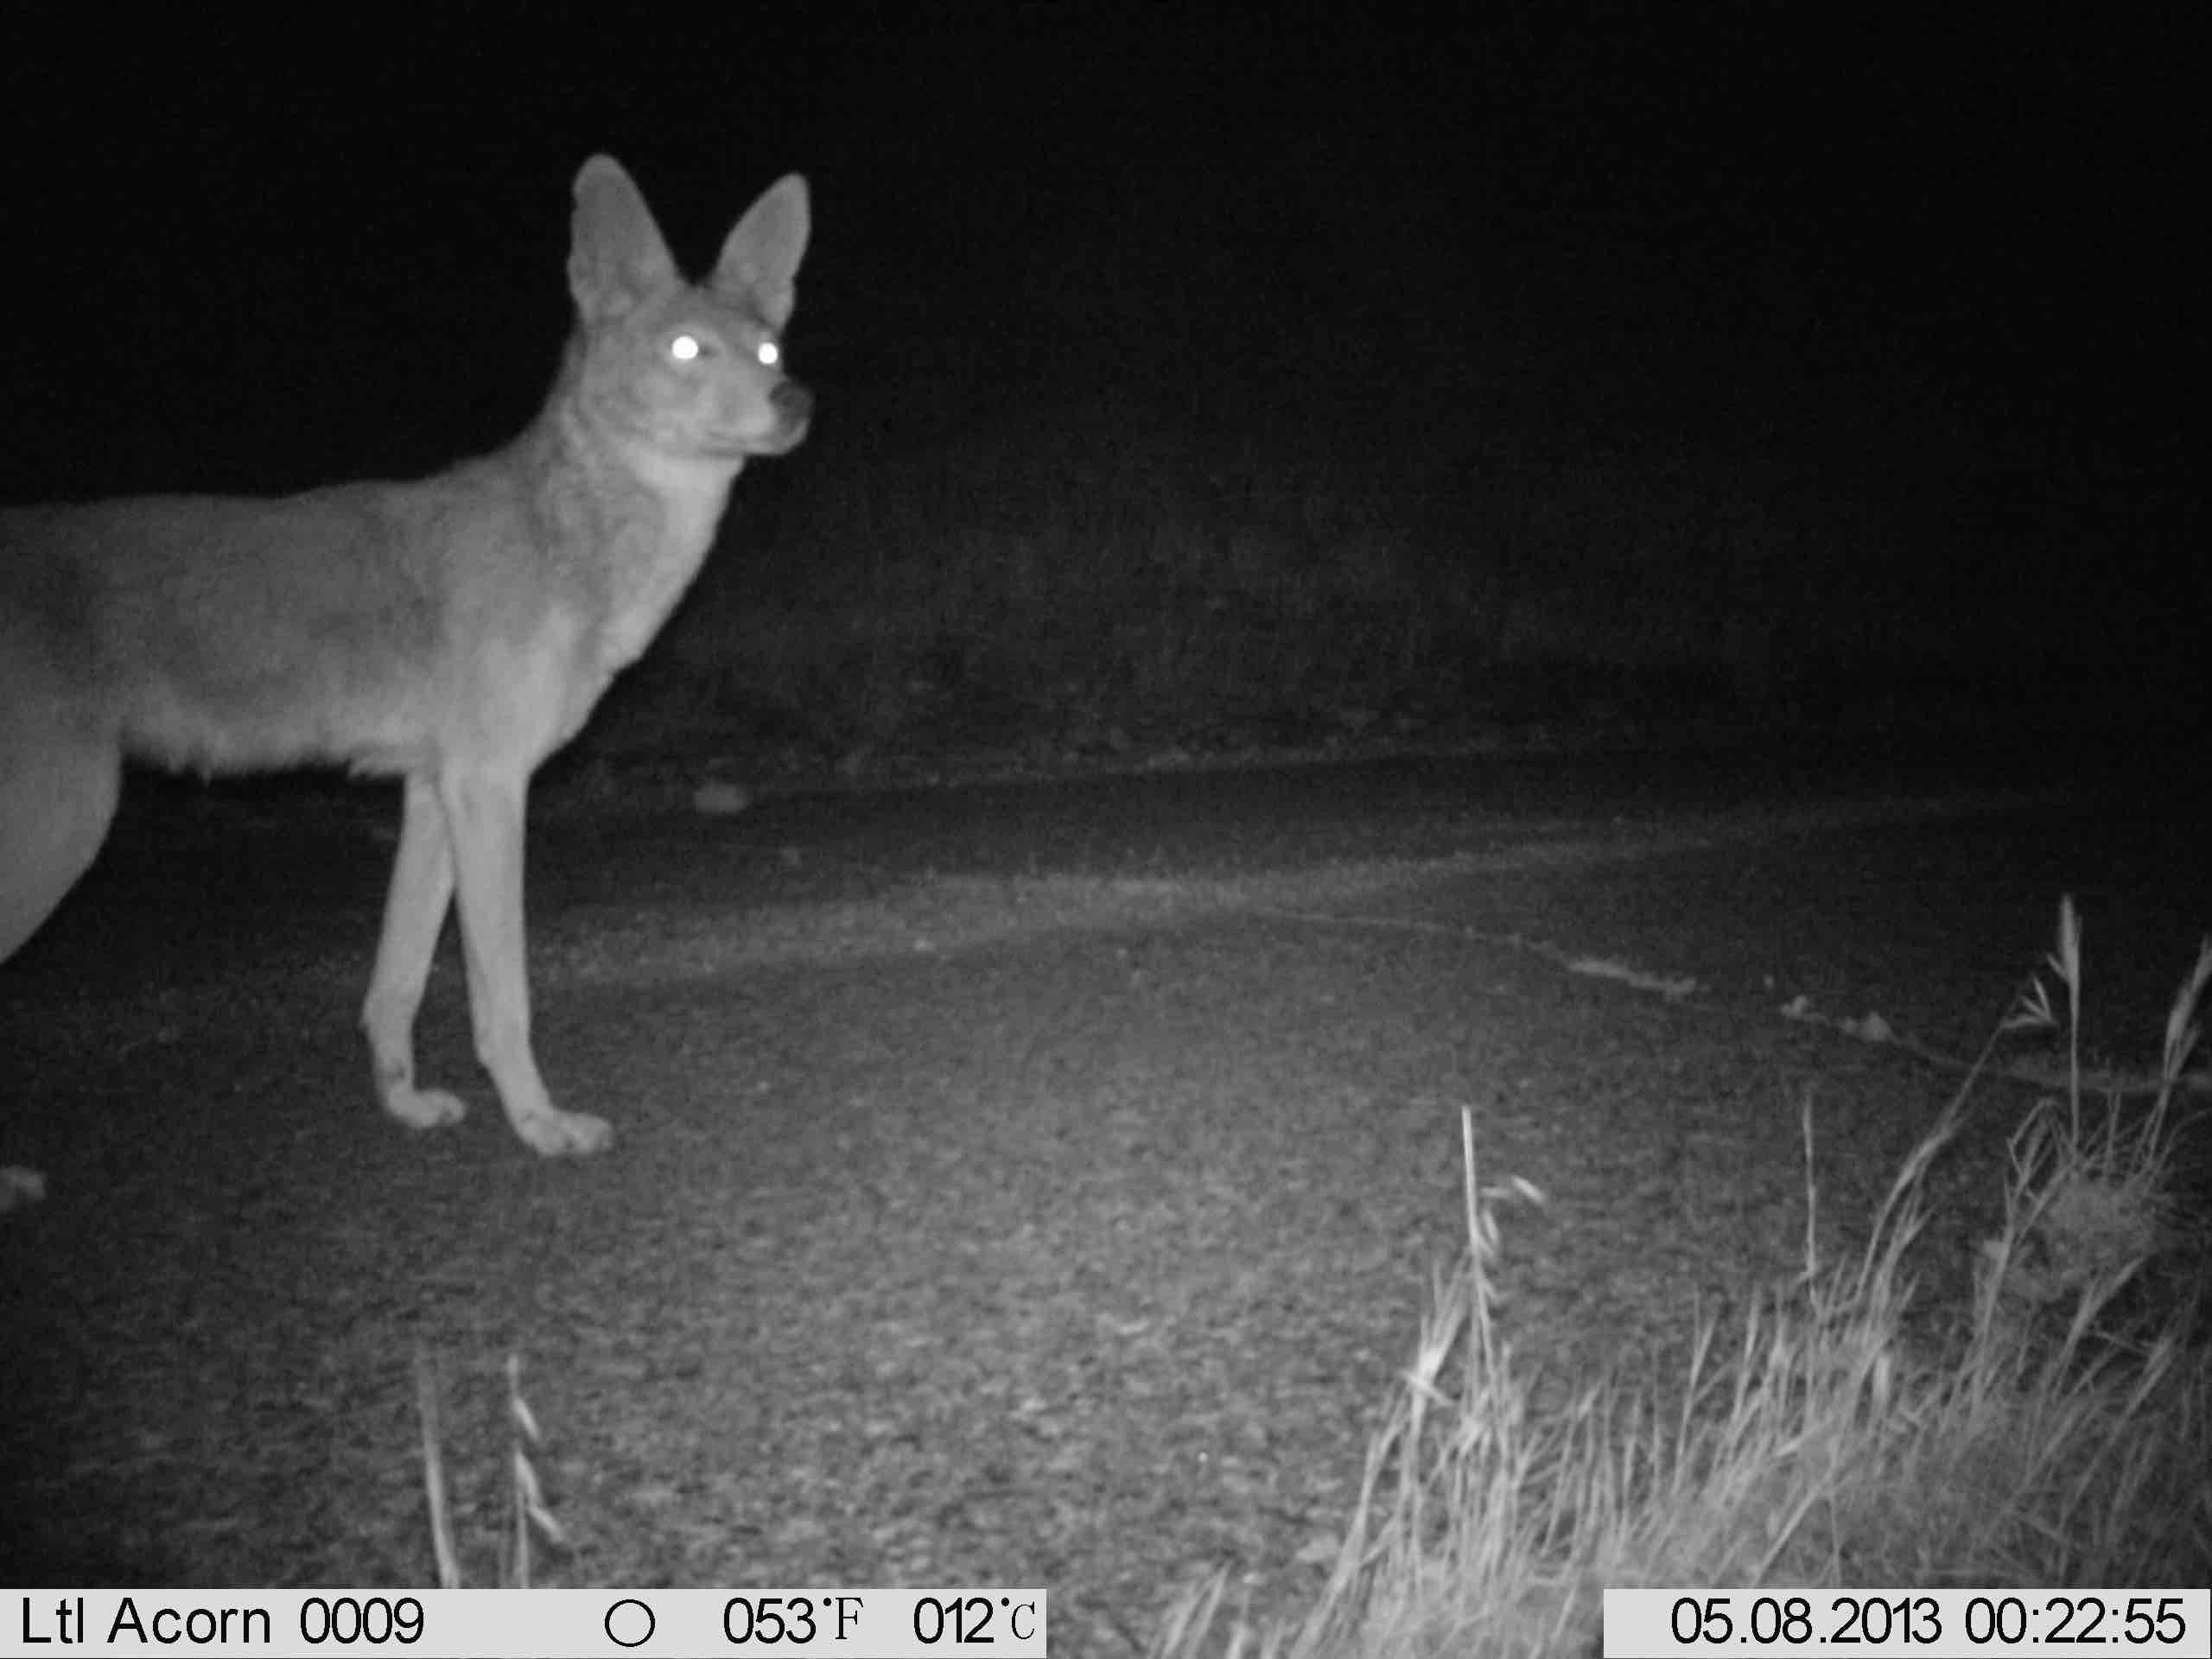
\includegraphics[width=.8\linewidth]{iwildcam_sample.jpg}
  \caption{Camera-trap sample}
\end{subfigure}%
\begin{subfigure}{.5\textwidth}
  \centering
  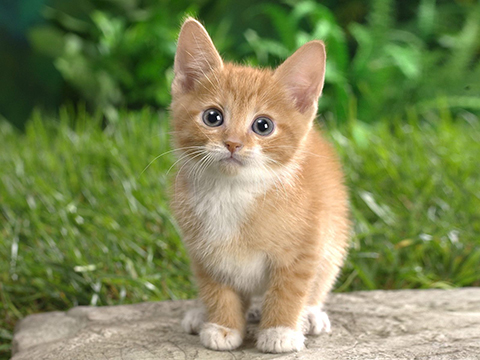
\includegraphics[width=.8\linewidth]{imagenet_sample.jpg}
  \caption{ImageNet sample}
\end{subfigure}
\caption[Camera-trap vs professional photography]{Example showing the differences between camera-trap image and professional photograph quality image}
\label{fig:camtraprealcam}
\end{figure}

Often, the images taken by camera trap are not free of right, causing a huge difference in quantity of publicly available datasets compared to general images datasets.

Transfer learning is an interesting solution when there is a lack of the specific data we want to train on.
Used by many\cite{feature_learning_bengio}\cite{decaf_feature}\cite{transfer_learning_bengio}\cite{dl__imagenet_seregenti_gomez}\cite{dl_imagenet_seregenti_norouzzadeh}, usually pre-training a model with ImageNet or similar general dataset then fine tuning with camera trap datasets like iWildcam and such.

\pagebreak\section{Conclusion}

Classification and detection are useful for wildlife monitoring, but action classification and other "exotic" tasks may be interesting in the future.
The advantage of object detection over classification is to know the position of the objects as well as to have several results per image, that's why I chose to focus on detection in the rest of this work 

\chapter{Implementation}
\section{Methodology}

As a reminder of the objective, there are camera traps that produce images and videos, ecologists want to have statistics on species to prevent their extinction.
At the moment, they recognize and count species manually, spending hours watching videos and photos, it takes a lot of time and is therefore very expensive.

The solution is to automatize this process with computer vision, this must meet the "four easy constraints":
\begin{itemize}
    \item Easy to deploy because ecologist usually don't have much computer science knowledge.
    \item Easy to maintain because we don't want something that need 10 hours/day monitoring if anything went wrong.
    \item Easy to scale, being able to handle either 1000 images / month or 1 000 000 images / month.
    \item Easy to price, having a fully transparent estimation of the different costs.
\end{itemize}

\pagebreak\subsection{Existing solutions}
\subsubsection{Microsoft Camera trap}
Microsoft AI for Earth propose a set of tools and algorithms especially designed for camera traps monitoring\cite{microsoft_camera_trap}.

It goes from data parsing scripts, pre-trained models on camera-trap images or web interfaces to use their models ...

An example of the model has been developed (see Figure ~\ref{fig:microsoftcamtrap}).

\begin{figure}[H]
\centering
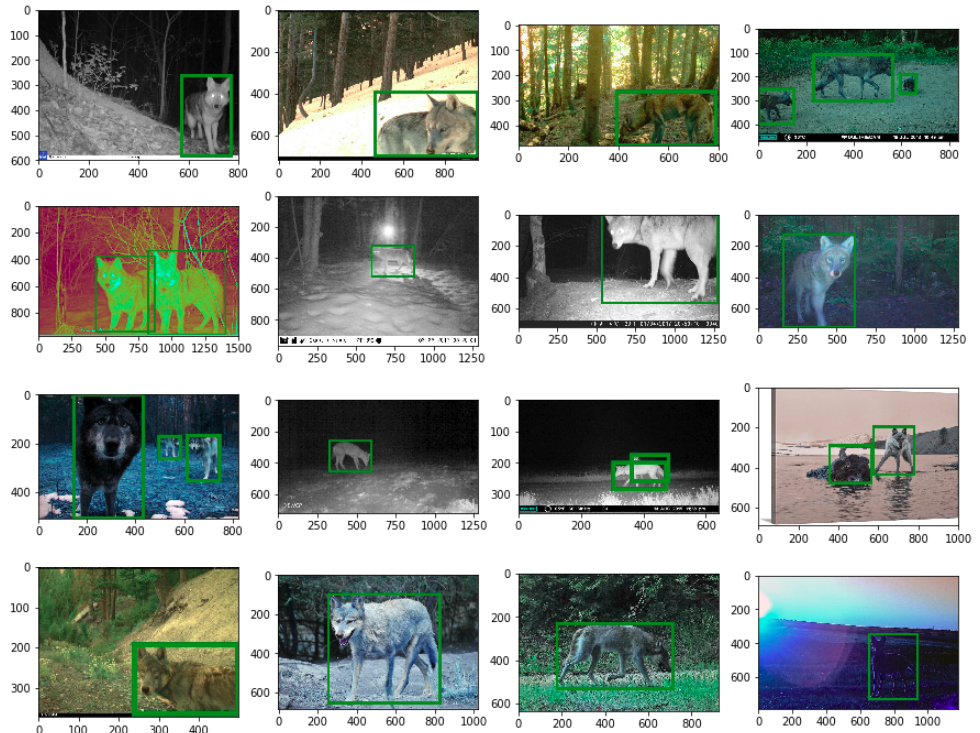
\includegraphics[width=.7\linewidth]{wolves_detected.png}
\caption{Example usage of Microsoft's camera trap model. \href{https://gist.github.com/louis030195/b64ba5a839c46c2ab0bf9451477a97df}{Source}}
\label{fig:microsoftcamtrap}
\end{figure}

This solution is not usable in production, it is a bit messy and no clear direction is given.
\subsubsection{Google DeepMind camera trap}
DeepMind, one of the lead actor in artificial intelligence research, the author of the major breakthroughs in AI, such as AlphaGo\cite{alphago}, AlphaStar\cite{alphastar} and much more are begining to take an interest in accelerate ecological research using machine learning\cite{deepmind_camera_trap}.
Their recent announcement is nevertheless rather vague, just an article and no code is available, they seems to work on training algorithm on the Seregenti Snapshot datasets.

Their solution will probably be interesting but not available in the short term

\subsection{Considered solutions}
Running a dedicated server is hard to deploy, it requires the implementation of containers, container-orchestration pipelines and other infrastructure tools.
To maintain it properly you also need to develop additional monitoring tools in order to keep track of its state.
It is also difficult to scale due to the work required on hardware side and finally the price can still be high.

With cloud providers (Amazon, Google, Microsoft, DigitalOcean ...) no need to worry about infrastructure, hardware, easy to deploy, maintain, scale and relatively price transparent.

We use Google Cloud Platform as a choice of experience, long-term potential and machine learning and big data orientation.


\pagebreak\section{Technologies}
\subsection{Machine learning}
Python has been chosen because it is the most popular programming language for machine learning\cite{python_machine_learning} due to numerous advantages:
\begin{itemize}
    \item Machine learning, vectors, math, visualisation libraries
    \item Massive community
    \item Machine learning frameworks
    \item Fast results
\end{itemize}

Next, usually the choice of framework have to been done between the most popular: Google's Tensorflow\cite{tensorflow} or Facebook's Pytorch\cite{pytorch}.

Both are open-source, the most important difference between the two is the way these frameworks define the computational graphs. While Tensorflow creates a static graph, PyTorch believes in a dynamic graph.
It means that Tensorflow is more difficult to learn at the moment, but Tensorflow will soon be released as 2.0 and it will be possible to create dynamic graph like Pytorch.
Tensorflow has way bigger community, more tools (Tensorboard, Tensorflow-serving ...).
Also it is obviously easier to use Google services with Tensorflow than Pytorch, for all these reasons Tensorflow has been chosen.

\pagebreak\subsection{Google Cloud Platform}
Google Cloud Platform is the platform that brings together Google's various cloud services. 
The Google Cloud Platform is a suite of cloud services offered by Google. The platform includes various cloud services for computing, storage, networking, Big Data, machine learning, Internet of things, security, cloud management and application development that are directly launched on Google's servers.

\subsubsection{Advantages}

Like all cloud platforms, Google's platform has the advantage of sparing companies the management of an infrastructure, server provisioning and network configuration. In addition, Google also highlights the evolutionary aspect of its infrastructure. Constantly updated and optimized, the platform benefits from Google's expertise and is efficient, economical and secure.

With the fully managed, server-less computing system, users can move from prototype to global production without worrying about capacity, reliability or performance. Other strengths of the Google Cloud Platform include a data center backbone network composed of thousands of kilometers of fiber optic cables combined with an advanced networking solution and edge caching services to deliver extreme performance.

\subsubsection{Services}

\begin{figure}[H]
    \centering
    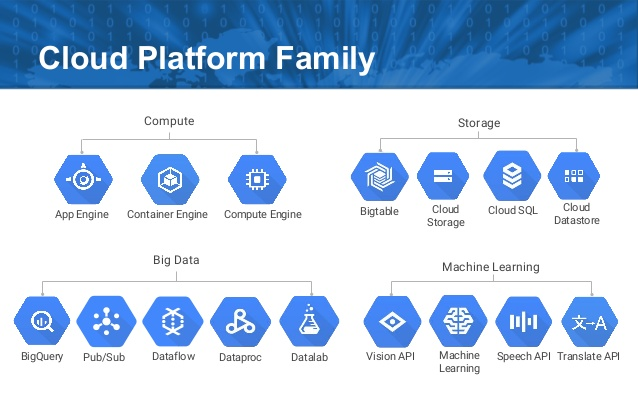
\includegraphics[scale = 0.55]{google-cloud-platform-services.jpg}
	\caption{Google Cloud Platform services}
	\label{fig:gcp}
\end{figure}


The Google Compute Engine is an Infrastructure as a Service (IaaS) that allows users to launch instances of virtual machines. This allows them to run their workloads on the cloud (see Figure ~\ref{fig:gcp}).

\begin{itemize}
    \item The Google App Engine is a Platform as a Service (PaaS). It allows software developers to access a scalable hosting offer. Developers can use an SDK to develop software that is compatible with the App Engine.
    \item Google Cloud Storage is a cloud storage platform designed to store large unstructured data sets. Google also offers database storage options, such as the Datastore for NoSQL storage, or CloudSQL for MySQL. We also find the native database Bigtable.
    \item The Google Container Engine is a management and orchestration system for Docker containers running on Google's public cloud. This system is based on the Google Kubernetes container orchestration engine.
The Google Cloud Platform also offers application development and integration services. For example, Cloud Pub/Sub is a real-time messaging service that allows messages to be exchanged between applications. Similarly, Endpoints allows developers to create services based on RESTful APIs and make these services very accessible.
\end{itemize}


\subsubsection{Other services}

Google also offers higher-level services on its Cloud platform, such as those dedicated to Big Data and Machine Learning. Google's Big Data services are used to process and analyze data. Google BigQuery allows you to search for data sets of several terabytes, for example. Dataflow is a data processing service designed for data analysis, extraction, transformation and loading. Dataproc offers Apache Spark and Hadoop services for Big Data processing. It also integrates the databases of Cassandra and MongoDB.

In terms of artificial intelligence, Google offers its Cloud Machine Learning Engine(Google Cloud AI Platform), a managed service that allows users to develop and train Machine Learning models. Different APIs are also available for the translation and analysis of speech, text, images or videos.
AI Platform allow to deploy any model in the Tensorflow SavedModel format, while the different API such as Video Intelligence is simple to use but is, at the moment, only for general use cases, for example it won't we suitable for camera-trap images.

\subsubsection{Prices}

Like most cloud service providers, Google Cloud Platform pricing is based on a pay-as-you-go (pay-per-use) business model, which means that users pay according to the resources they consume. Resource consumption is accurately calculated to the minute. According to Google, the platform's rates are on average 60\% lower than those of other providers\cite{gcp_pricing}.

The other advantage of this model is that users do not have to pay upfront fees. Similarly, billing ends as soon as the user ceases to use the services without having to pay termination fees. For Google Compute Engine and Cloud SQL services, Google also offers an automatic discount system of up to 30\% on the most used workloads. Rates vary between the different services and should therefore be consulted on a case-by-case basis on the official website.

\pagebreak\subsection{Front end}
We have chosen to use Javascript, which is the most popular language for the front end.
Front end web development is a field that is evolving very quickly and solutions are quickly becoming obsolete.

Especially, we use Lit-Element which is created to support a component-oriented approach to front-end Web development.

Lit-Element is an open-source JavaScript library used to develop Web applications using Web components. Created by Google developers and contributors on GitHub.

The advantage of Lit-Element is that you don't need to know in detail how it works unlike popular front end heavy frameworks such as Angular, React, Vue and others.

\pagebreak\section{Online versus Batch predictions}
AI Platform offers two methods for obtaining predictions from trained models: online prediction and batch prediction. In both cases, you transmit input data to a machine learning model hosted in the cloud and obtain inferences for each instance of data (see the differences in Figure ~\ref{fig:onlinebatch}).

\begin{figure}[H]
    \centering
    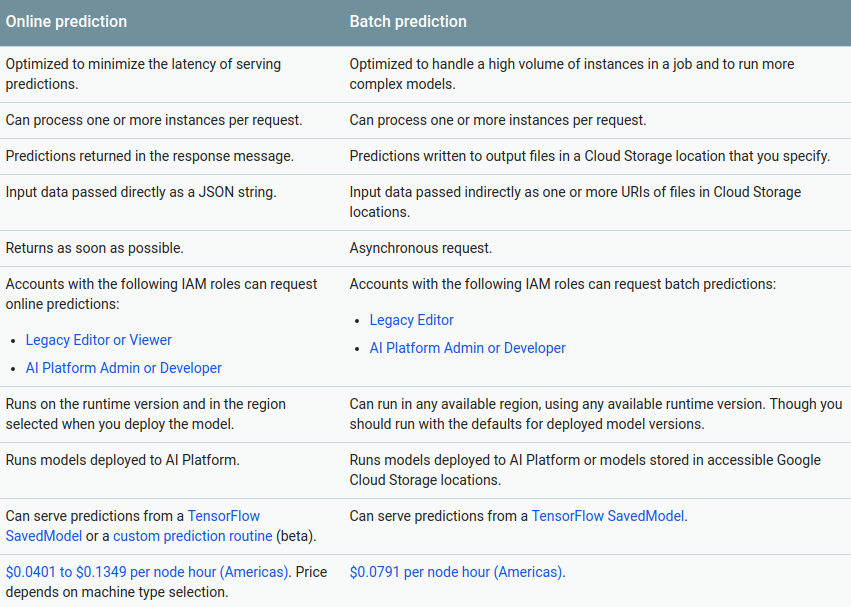
\includegraphics[scale = 0.5]{online_vs_batch.png}
	\caption{Online versus batch predictions. \href{https://cloud.google.com/ml-engine/docs/tensorflow/online-vs-batch-prediction}{Source}}
	\label{fig:onlinebatch}
\end{figure}

It is generally preferable to use online prediction to make requests in response to an application entry or in other situations where rapid inference is required.

Batch prediction is ideal when processing accumulated data, when you do not need immediate results. For example, a periodic task that makes predictions from all the data collected since the last task.

You must also make your decision taking into account potential variations in the cost of prediction.

Here we obviously chose batch prediction because our goal is to have statistics of species over long times, we don't need to have instant result, the user will drop big amount of videos / photos that will be processed.

\subsubsection{Latency of batch prediction}
If you use a simple model and a small set of input instances, you will find that, to complete identical prediction requests, there is a considerable difference in the time required if online prediction is used compared to batch prediction. A batch task can take several minutes to complete predictions that would be returned almost instantly by an online request. This is a side effect of the difference between the infrastructures used by the two prediction methods. AI Platform allocates and initializes resources for a batch prediction task when you send the request. The online prediction is usually ready to be processed at the time of the request.

\pagebreak\section{Architecture}

The ultimate high-level objective of this is to allow users to easily upload visual data in a secure and privacy preserving manner and get useful insights about wildlife populations through visualisation like graphics, heat maps ...


The core of this architecture is powered by Google Cloud AI Platform, a service that allow quickly and cost-effectively deployment of machine learning models to production. 
Google Cloud AI Platform has nevertheless a few flaws, such as the unavailability of GPUs for inference which are very powerful for computer vision\cite{gpu_cnn}, the lack of documentation or the limit of 250mb models.

The second most important part is Google Cloud App Engine, which allow to create and deploy an application on a fully managed server-less platform. It allow easy scaling without having to worry about managing the underlying infrastructure. 

Then come the storage component, Google Cloud Storage is a web-based RESTful online file storage service for storing and accessing data on the Google Cloud platform infrastructure. This service combines the performance and scalability of Google's cloud with advanced security and sharing features.

To persist data, a NoSQL solutions of Google is used: Cloud Datastore which offers great scalability for the applications. 

This tool automatically manages the partition and replication of data allowing a durable and highly available database that can dynamically evolve to absorb the load of the applications. 

Cloud Datastore offers a multitude of features, such as ACID transactions, SQL queries, indexes and more.

Lastly, multiple small event-triggered codes have been deployed through Google Cloud Function, GCF is a server-less runtime environment for creating and connecting cloud services. 

Cloud Functions are usually used to write simple and single-use functions that are attached to events issued by the cloud infrastructure and services.

The Cloud function is triggered when an observed event is triggered. The code runs in a fully managed environment. There is no need to provision the infrastructure or worry about server management.

\pagebreak
Multiple cloud pipelines have been considered, their advantages and disadvantages have been studied carefully, where some infrastructure fails, where it succeed.

To conduct such a process, a list of use cases needed to be put down:

\begin{enumerate}
    \item I want to send an image and have the prediction right away
    \item I want to send 1000 images and have the prediction as soon as available
    \item I changed my model, I want to make all the predictions again
    \item I want to send a video, and have the predictions right away
    \item I want to send 100M images and have the predictions as they happen, knowing how long it will be before I have the predictions and how much it will cost me
    \item I want to send 1000 videos and know time and cost
    \item I want to automatically send videos from camera trap device
    \item I have 1000 cameras trap that will send videos, how much it will cost me
\end{enumerate}

Of course, there are probably more cases, but it is at least a few simple cases where an architecture can have bottlenecks.


\pagebreak\subsection{Pipeline version 1}

\begin{figure}[H]
    \centering
    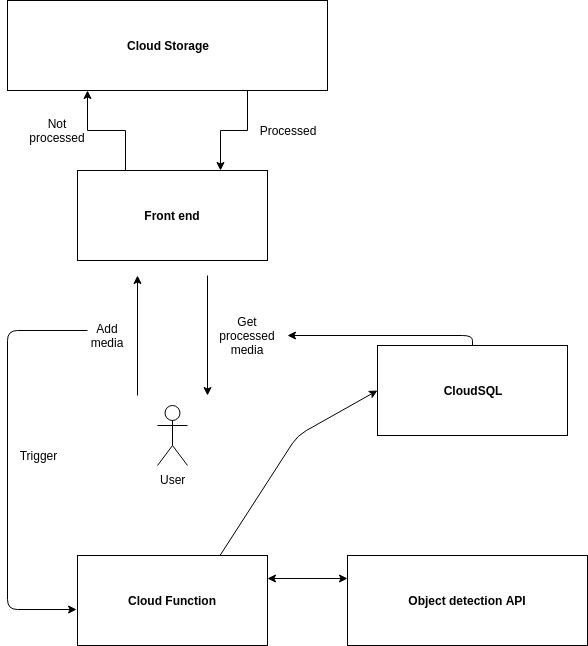
\includegraphics[scale = 0.4]{gcp_pipelinev1.png}
	\caption{GCP pipeline version 1}
	\label{fig:pipelinev1}
\end{figure}

In this version, data would be stored in Google Cloud Storage, the front end would be hosted on a Google Cloud App Engine using NodeJs programming language.

A Golang-written (for performance) cloud function will be triggered when data have been added, calling the AI Platform's hosted model to process it (see ~\ref{fig:pipelinev1}).

\pagebreak
It is a first nice simple solution in theory, but in practice it encounters few problems
\begin{enumerate}
    \item No queue (if you add 100 images, the cloud function will ask a lot to AI Platform, it should wait the end of each processing through a queue)
    \item On the cloud function side again, Python has way more tools to process images, machine learning ... than Golang which is really focused on server side communication
\end{enumerate}

Regarding the use cases here is how it goes for this version:
\begin{enumerate}
    \item Works and on average shouldn't take more than a few seconds maximum: success
    \item The first images will be processed effectively, then a lot of errors and crashes will occurs, overloading the model: fail
    \item All images will have to be uploaded again: fail
    \item This version doesn't handle videos: fail
    \item Everything will crash, no estimations: fail
    \item This version doesn't handle videos: fail
    \item This version doesn't handle videos: fail
    \item This version doesn't handle videos: fail
\end{enumerate}

\pagebreak\subsection{Pipeline version 2}
\begin{figure}[H]
    \centering % TODO UPDATE IMG
    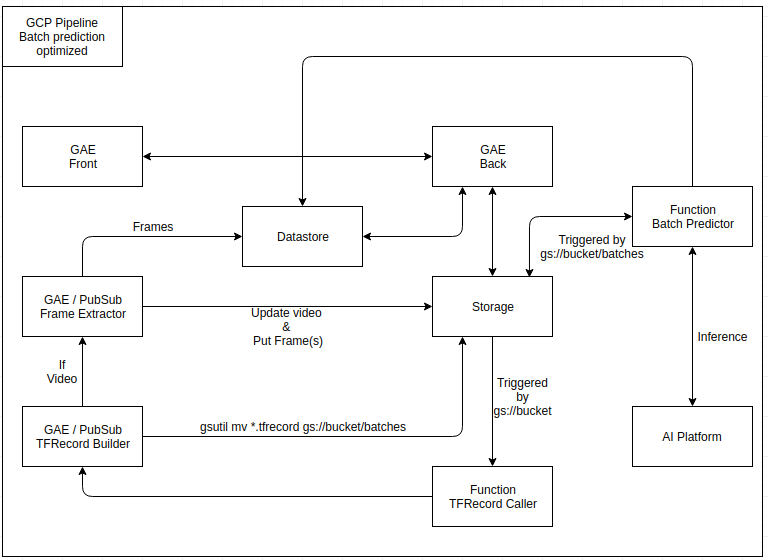
\includegraphics[scale = 0.5]{gcp_pipeline2.png}
	\caption{GCP pipeline version 2}
	\label{fig:pipelinev2}
\end{figure}

The major change here is the use of batch prediction which takes a different kind of input.
Online prediction usually either require an input four dimensions vector of the shape (-1, -1, -1, 3) (first dimension is the number of images, so in online it is always 1, second dimension is the width, third the height and lastly the channel).

Example of 4-d vector input in Python, converting a Numpy array into a serializable list
\begin{lstlisting}[language=Python]
{"inputs": img.tolist()}
\end{lstlisting}

Either it can accept a byte string of the shape (-1), encoded for example in Python:
\begin{lstlisting}[language=Python]
{"inputs": base64.b64encode(jpeg_data)}
\end{lstlisting}

\pagebreak
Batch prediction require the sames types of inputs but stored in a file put in Google Cloud Storage, the file has either a JSON format, a TFRecord format which is the archive format of Tensorflow or a TFRecord GZipped.

TFRecord is way lighter than JSON so an implementation of a TFRecord builder has been developed and deployed in an App Engine.

The second advantage of this version over the first is the introduction of queues through Google Cloud PubSub which handle the communications between Google Cloud services, making concurrent-running components less likely to crash.
This version also includes some more little cloud functions and is more modular (see Figure ~\ref{fig:pipelinev2}).

The problem in this version is the disappearing of online predictions which can be useful for fast predictions, also too many App Engine are used while simple cloud functions would have been enough.

Regarding the use cases here is how it goes for this version:
\begin{enumerate}
    \item This version doesn't handle online prediction: fail
    \item Works and on average shouldn't take more than a few minutes maximum: success
    \item All images will have to be uploaded again: fail
    \item This version doesn't handle online prediction: fail
    \item Possible but no estimations: success
    \item Possible but no estimations: success
    \item Possible, depending in the amount of scaling required: success
    \item Possible, depending in the amount of scaling required but no estimations: success
\end{enumerate}
\pagebreak\subsection{Pipeline version 3}
\begin{figure}[H]
    \centering
    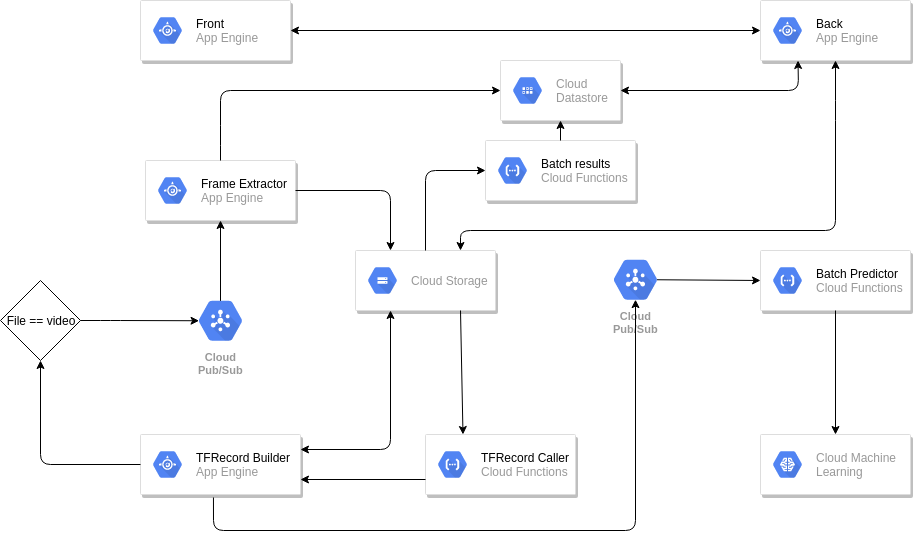
\includegraphics[scale = 0.4]{gcp_pipelinev3.png}
	\caption{GCP pipeline version 3}
	\label{fig:pipelinev3}
\end{figure}

The third version is quite similar to the previous one, some simplifications have been done (see Figure ~\ref{fig:pipelinev3}).

It still lacks online predictions and overuse Google App Engine which are quite expensive.

Regarding the use cases here is how it goes for this version:
\begin{enumerate}
    \item This version doesn't handle online prediction: fail
    \item Works and on average shouldn't take more than a few minutes maximum: success
    \item All images will have to be uploaded again: fail
    \item This version doesn't handle online prediction: fail
    \item Possible but no estimations: success
    \item Possible but no estimations: success
    \item Possible, depending in the amount of scaling required: success
    \item Possible, depending in the amount of scaling required but no estimations: success
\end{enumerate}

\pagebreak\subsection{Pipeline version 4}
\begin{figure}[H]
    \centering
    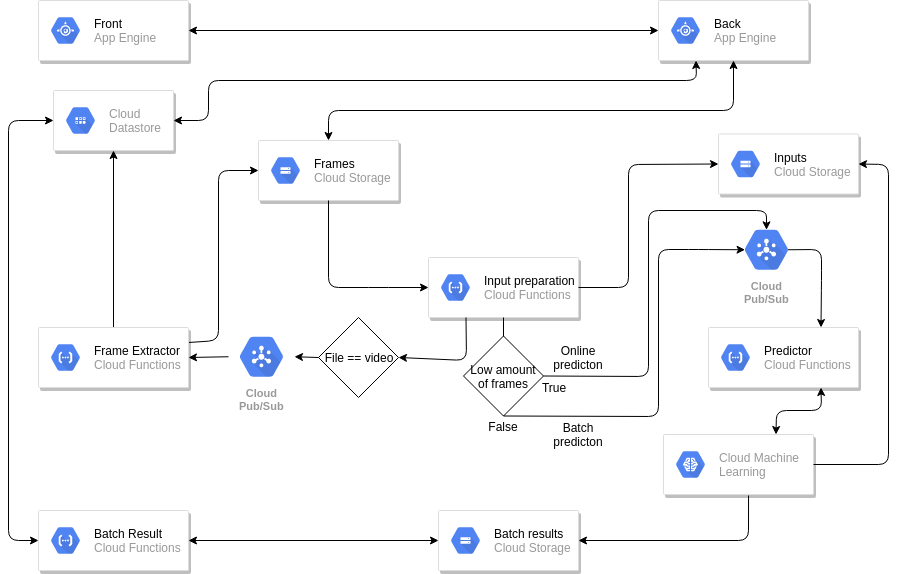
\includegraphics[scale = 0.5]{gcp_pipelinev4.png}
	\caption{GCP pipeline v4}
	\label{fig:pipelinev4}
\end{figure}

The fourth version have evolved through his predecessor, fixing bottlenecks, improving the overall pipeline, handling both batch and online predictions (see Figure ~\ref{fig:pipelinev4}).

The choice between online and batch prediction is customizable by the user, by default batch prediction are preferred over a certain threshold of data to process, under this threshold online predictions are called for fast predictions.

\pagebreak
Regarding the use cases here is how it goes for this version:
\begin{enumerate}
    \item Works and on average shouldn't take more than a few seconds maximum: success
    \item Works and on average shouldn't take more than a few minutes maximum: success
    \item All images will have to be uploaded again: fail
    \item Works and on average shouldn't take more than a few minutes maximum: success
    \item Possible but no estimations: success
    \item Possible but no estimations: success
    \item Possible, depending in the amount of scaling required: success
    \item Possible, depending in the amount of scaling required but no estimations: success
\end{enumerate}

In the end, the only lacking features are price and time estimations before and after upload and the change of model, both are easy to implement and shouldn't take more than a few hours, the biggest part of the architecture was the front end, back end and make everything communicate well together, in addition of the fact AI Platform batch jobs require 6 minutes to boot at cold start, so it took a while to test everything.

\pagebreak\subsection{Components}

Now all components of this final pipeline will be described in detail.

\textbf{Front} component is in charge of directly interfacing with user, it allows to upload images and videos, get prediction results, see statistical graphics about the occurrences of animals over time and space.
It communicates with \textbf{Back} to send images, retrieve predictions and statistics.
\textbf{Front} is implemented with Lit-Element as a single page application.

\textbf{Back} is a REST API implemented in JavaScript with Express package, it saves information about frames and predictions in \textbf{Cloud Datastore}. It stores images and videos in \textbf{Cloud Storage}.
It runs on App Engine so it can scales to any number of instances to handle higher traffic.

\textbf{Cloud Datastore} is a NoSQL database which stores frames, videos, predictions and detected objects, it is convenient to be able to iterate fast without having to define the schema of the database first.

\textbf{Cloud Storage} is a scalable filesystem to store large amount of files, it is used to store images, videos, batch predictions inputs and outputs.

\textbf{Frame extractor} is a cloud function that split videos into frames and store them in \textbf{Cloud Storage} and their metadata in \textbf{Cloud Datastore}.

\textbf{Input preparation} is responsible for building the input of both online and batch predictions from frames and storing it on \textbf{Cloud Storage}. It retrieves the frames from \textbf{Cloud Storage} and publish on \textbf{Cloud PubSub} queue.
It chooses between online or batch prediction based on different parameters to fulfill user needs, for example if the user has only few images to tag it makes sense to use online prediction, if he has ten thousands of videos it makes more sense to use batch prediction.

\textbf{Cloud PubSub} is used to limit the calling rate of batch and online prediction. It is useful because Google API are rate-limited to avoid waste of resource. 

\textbf{Batch prediction AI Platform} receive batch of frames and start a job which automatically scales in many workers and output the predictions efficiently for large number of frames, launching a job takes several minutes so it is not used for few frames.
Results are stored in \textbf{Cloud Storage}.

\textbf{Online prediction AI Platform} produces prediction for one frame with low latency, the result is available in the HTTP answer.

\textbf{Batch result} is a cloud function that update the predictions once they are done into \textbf{Cloud Datastore}.

\pagebreak\section{Data flows, number of operations : price \& time estimations}

In the last few years, people are still hesitating to dive in cloud providers like Amazon, Google, Microsoft with the fear of multiple concerns: losing control, security, data protection, performance and price.
The cloud services are usually difficult to estimate in price, here an example use case showing the consumption of storage and cloud operations using this solution in production is described.
The cost in term of storage, Datastore, ... is detailed in next parts

\subsection{Data \& Ops}
A typical use case would be: 
\begin{enumerate}
    \item Reach main page
    \item Upload a picture
    \item Back on main page to see the results (after a while of course)
\end{enumerate}

\subsubsection{Storage}
\begin{itemize}
    \item Two megabytes image
    \item One operation to store the image
\end{itemize}
\subsubsection{Datastore}
\begin{itemize}
    \item Storage of the annotation mapping approximately <= 1000 rows
    \item Two rows Frame entity (store, then update when prediction are ready)
    \item Predictions into Prediction entity 1 row
    \item Objects detected into Object entity < 50 rows (being large)
    \item One operation put class mapping
    \item One operation put frame
    \item One operation prediction
    \item One operation put objects
\end{itemize}
\subsubsection{Function}
\begin{itemize}
    \item One operation input preparation
    \item One operation prediction
\end{itemize}
\subsubsection{PubSub}
\begin{itemize}
    \item One message being stored and published
\end{itemize}
\subsubsection{App Engine}
\begin{itemize}
    \item Two operations frontend rendering main page
    \item One operation front render upload page
    \item One operation back call frames list
    \item One operation back call frames upload
\end{itemize}
\subsubsection{AI Platform}
\begin{itemize}
    \item One operation online prediction
\end{itemize}

\pagebreak\subsection{Price \& Time}
%https://cloud.google.com/products/calculator/#id=8c3bc8ef-79f9-45da-a7f4-eec8337c3cb5

\begin{figure}[H]
    \centering
    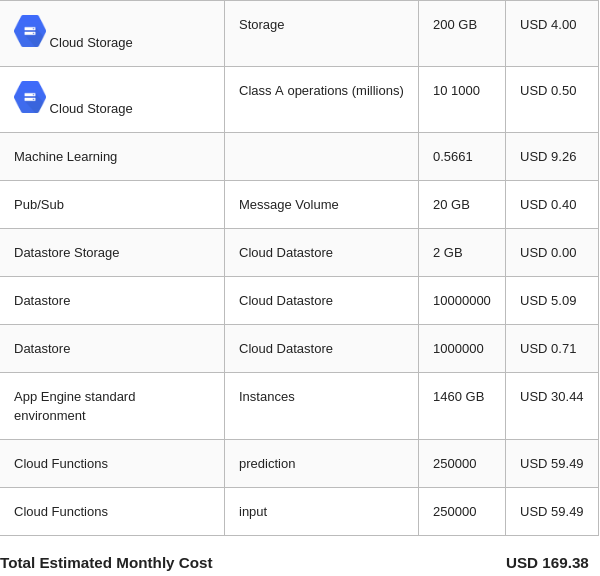
\includegraphics[scale = 0.65]{price_estimation.png}
	\caption{Example price estimation. \href{https://cloud.google.com/products/calculator/\#id=8c3bc8ef-79f9-45da-a7f4-eec8337c3cb5}{Source}}
	\label{fig:priceestimation}
\end{figure}

You can see on Figure ~\ref{fig:priceestimation} the largely estimated price for 100 000 images per month.

This price can probably be highly lowered since no optimization has been done and the "default" and even non needed higher configurations of services have been chosen (2 permanently running App Engine instances, high memory capacity for cloud functions ...).

In addition, creating this estimation helped to recognize where the solution can be optimized to reduce the overall cost.

\pagebreak\section{Statistics}

Statistics based on graphs and other visualizations are available to monitor the evolution of species and their behaviour, some interesting information are:
\begin{itemize}
    \item Occurrence of species over time and zone (plots, charts, histograms, heatmap ...)
    \item Co-occurrence of species, showing the link between them
\end{itemize}

Once a certain amount of data has been generated, one can even imagine using predictive models, from simple linear regression, random forests, boosted trees to neural networks for prevention.

Algorithms to detecting anomalies such as principal component analysis could also help analysing the changes and alert ecologists, for example if a species is suddenly in a sharp decline, this could potentially be the cause of poaching.

Another example would be the strong growth of an invasive mosquito species that would be automatically detected by such algorithms above a certain threshold and would prevent the competent authorities


\pagebreak\section{Used models}

Here a choice needed to be made to take the best model in term of speed / accuracy (mAP) tradeoff AND less than 250mb model to respect AI Platform constraint.

\begin{figure}[H]
    \centering
    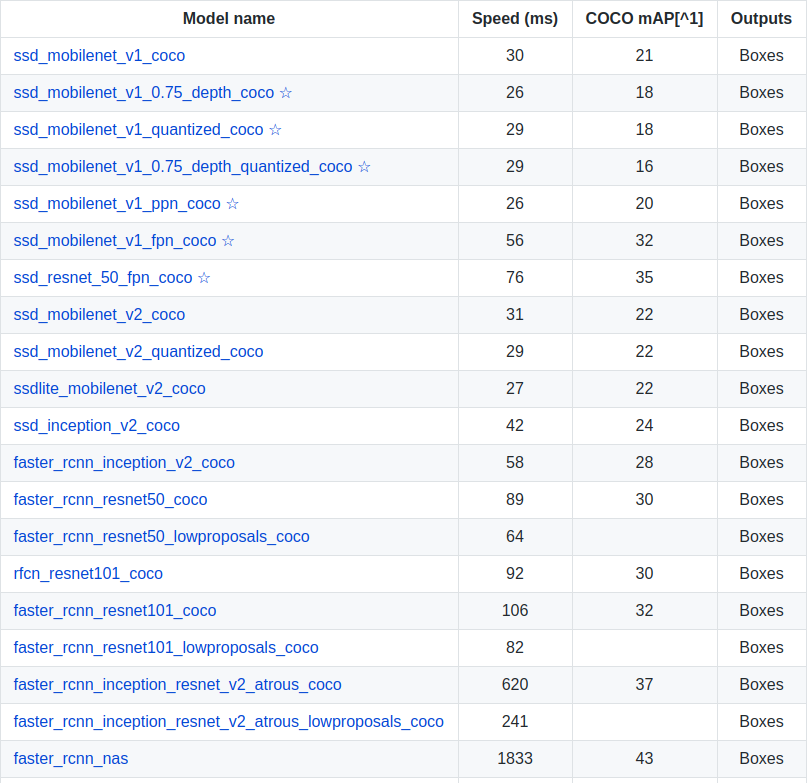
\includegraphics[scale = 0.5]{tensorflow_models_coco_models.png}
	\caption{COCO trained models, speed / accuracy tradeoff. \href{https://github.com/tensorflow/models/blob/master/research/object_detection/g3doc/detection_model_zoo.md}{Source}}
	\label{fig:tfmodels}
\end{figure}

Another constraint was the fact that changing the graph makes the file size grow.

Faster RCNN NAS is the most accurate model obviously because of its neural architecture search algorithm, but 1833 is very high compared to others (see Figure ~\ref{fig:tfmodels}).
An interesting one was SSD ResNet 50 FPN, ending around 180mb after the graph modification.

\pagebreak\section{Performances}

With AI Platform configured with 72 max workers, 1 CPU core and a SSD ResNet50 FPN model, it takes about 20 minutes to process a batch of 10 000 images with a resolution of 100x100 (see Figure ~\ref{fig:10kjob})

\begin{figure}[H]
    \centering
    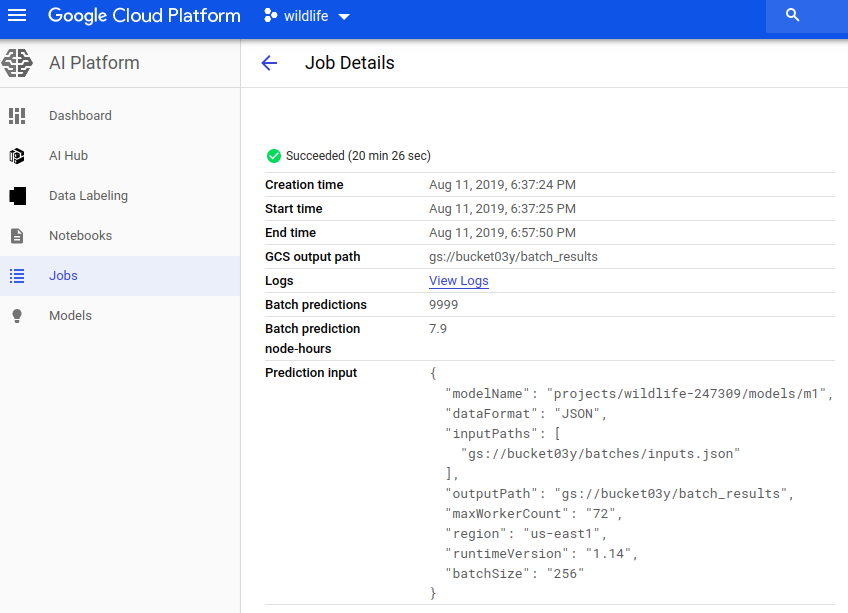
\includegraphics[scale = 2]{10k_job.png}
	\caption{Batch prediction job of 10 000 images}
	\label{fig:10kjob}
\end{figure}

On 	~\ref{fig:10kjob} you can see that in this context it has cost 7.9 node hours at the price of \$0.0791\footnote{see https://cloud.google.com/ml-engine/docs/pricing} which makes a total price of about \$0.6.

\pagebreak\section{Optimization}
In the world of machine learning, the optimization of training is receiving a lot of attention. There is much less information available on inference optimization. 

Yet, isn't serving prediction models the point of ML ?

Serving performance can have a significant impact on the ML value for your use case. Indeed, the cost of inference can be a major factor in the total return on investment of an ML application.

\subsection{Latency (and size) count}
When it comes to optimizing production models, we are mainly concerned with three things:
\begin{itemize}
    \item Model size
    \item Prediction speed
    \item Prediction rate
\end{itemize}

When serving ML, the size of the model is important. Of course, smaller models use less memory, less storage and network bandwidth, and they load faster. In some cases, hardware memory constraints or service limitations may impose a limit on the size of the model. For example, the Machine Learning Engine service on Google Cloud (GCP AI Platform) sets a default size limit of 250 MB for models. 

When we use hardware acceleration for prediction purposes, we must ensure that our model fits into the memory of the acceleration device. The size of the model has a particular impact in situations where we serve it on a peripheral or mobile device with limited capacity. We want the model to be downloaded as quickly as possible, using as little network bandwidth as possible and using as little memory and storage capacity as possible.

Prediction speed is another metric that is important. When we make our online inference, we generally want the results to be returned as quickly as possible. In many online applications, latency is critical to the user experience and application requirements. But we care about the speed of inference, even when we process our data in batches. The inference speed is directly related to the cost of the service, as it is directly related to the amount of computing resources required to make a prediction. The time required to make a prediction will always be a critical variable in any formula that measures the rate of prediction. 

Faster forecasts mean more prediction throughput on the same hardware, resulting in lower costs.
The prediction rate is a measure of the number of predictions that our system can make in a given time period. In addition to the prediction speed mentioned above, other system attributes are involved in determining throughput, including batch processing of forecasts, hardware acceleration, load balancing and horizontal scaling of service instances.


\subsection{Exported model formats in TensorFlow}
TensorFlow has several model serialization formats, but the most important ones to know are the GraphDef and SavedModel formats. 
\begin{itemize}
    \item The GraphDef format is a version of the ProtoBuf\cite{protobuf} serialization protocol, in text or binary form, that codes the definition of a TensorFlow graph. A GraphDef can also include the weights of a trained model, but it does not have to - the weights can be stored in separate control point files. 
    \item The SavedModel format combines a GraphDef with control point files that store weights, all gathered in a folder.
\end{itemize}


\subsection{Tools and techniques}
TensorFlow offers several techniques to reduce the size of a model and improve prediction latency.
Here are some of them:

\begin{itemize}
    \item Freeze: Convert variables stored in a SavedModel control point file to constants stored directly in the model graph. This reduces the overall size of the model.
    \item Pruning: Remove unused nodes in the prediction path and graph outputs, merging duplicate nodes and cleaning other node operations such as summary, identity, etc.
    \item Constant folding: Substitute the values of known constants in expressions at compile time in the sub-graphs of the model
    \item Batch standard folding: Fold the multiplications introduced in the batch normalization into the weight multiplications of the previous layer.
    \item Quantization: Convert floating point weights to lower accuracy, such as 16 or 8 bits.
\end{itemize}

For mobile deployment, there is also TFLite, which performs 8-bit quantification on mobile models.

TensorFlow offer a graph transformation tool to perform most optimizations, which is a C++ command line tool.

The Graph Transform tool is designed to work on models saved as GraphDef files in protobuf format. However, the SavedModel format is the most modern and most supported by other tools and services. This is the only format supported by Google Cloud AI Platform for prediction.
The optimization steps, as well as the model format transitions, are as follows:
\begin{enumerate}
    \item Freeze the exported model: SavedModel => GraphDef
    \item Optimize the fixed model: GraphDef => GraphDef
    \item Convert the optimized frozen model back: GraphDef => SavedModel
\end{enumerate}


\pagebreak\section{Other tools built}
All the tools are publicly available on the main Github repository.

\subsection{Inference graph modification}
Batch prediction on AI Platform cause a problem, when the prediction are done and written to a file, nothing give any information about which prediction is linked to which input.

To solve this problem, a tool to change the graph of the model needed to be developed.

Tensorflow offer a repository specific to models\cite{tensorflow_models}, many tools are available there to work with object detection graphs.
Tensorflow also make the possibility to display a graph through a command-line script.


\begin{figure}[H]
  \centering
  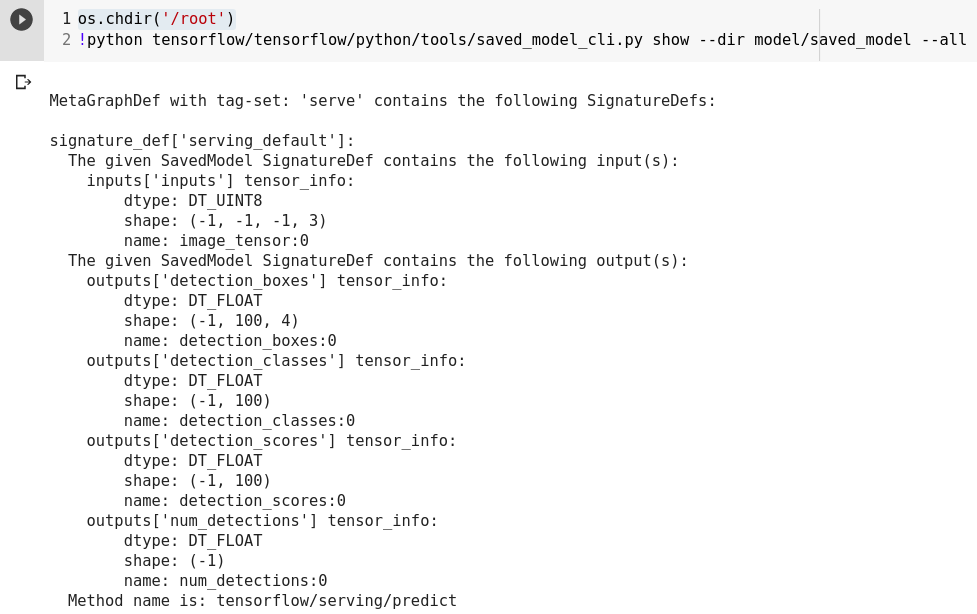
\includegraphics[width=1\linewidth]{initial_graph.png}
  \caption{Initial object detection graph}
  \label{fig:initialgraph}
\end{figure}

A Tensorflow object detection model's graph input and output is shown on Figure ~\ref{fig:initialgraph}.

\begin{figure}[H]
  \centering
  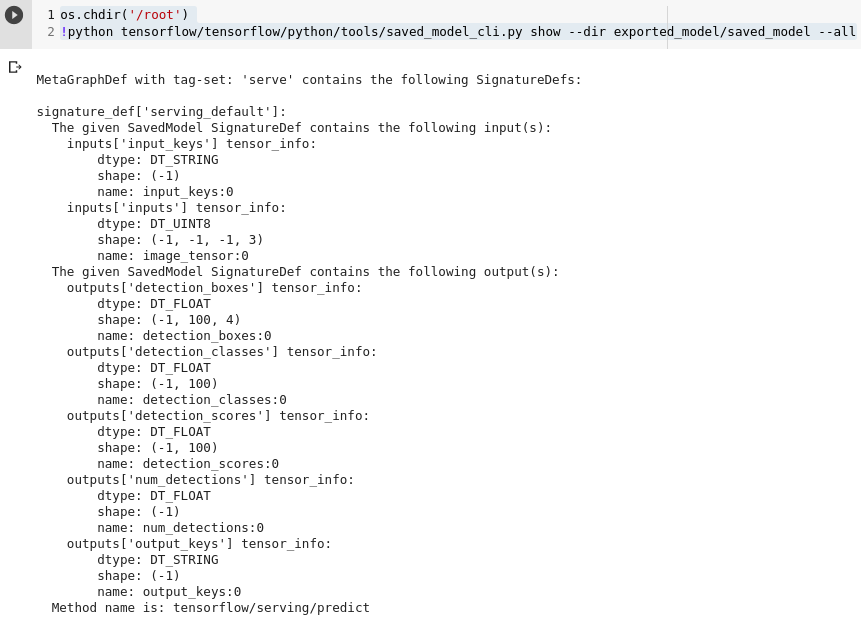
\includegraphics[width=1\linewidth]{modified_graph.png}
  \caption{Changed graph to handle keys}
  \label{fig:changedgraph}
\end{figure}

Then you can see on Figure ~\ref{fig:changedgraph} the modified graph with the input and output keys used to map an image to its prediction (E.g. I detected a cat at top-left ...)

A fork and modification of Tensorflow Models repository has been done\footnote{See https://github.com/louis030195/models} to allow such graph modification.

\subsection{Gitpod configurations}

The growth of cloud services made also available cloud development possible, an example of this is Google Colaboratory\cite{colab} which have been of great use but is only for Python, Gitpod\cite{gitpod} allows to develop in most languages.

A customised Docker configuration has been developed to allow ready-to-code environment in a click\footnote{see https://github.com/louis030195/vision-client}.


\chapter{Future Work}
\section{Individual species identification}
It could be as much interesting as useful to be able to differentiate a species from another, it could be used to track and understand some behaviours.
In order to implement such a thing a similar approach than face recognition algorithm could be used, previous work has been done on bear\cite{bearfacenet}, indeed facenet\cite{facenetoriginal} algorithm is adapted to this kind of task.

\section{New tasks}

In the solution we propose, only object detection is handled, in the future some more tasks could be setup, putting multiple models at disposal to the user.

\subsection{Video classification}
Video classification(action classification) in the field of wild life could be used to understand the behaviours of different species over time and space, while it's probably inaccessible now due to the lacks of data and being a less popular task, it can still be solved later by means of creating datasets specially designed and annotated for this.

\subsection{Pose estimation}
Pose estimation is the task to track an animal's every part of the body small movement in real time.
Of similar utility than video classification, it could help to understand species behaviour and interactions.
Again, this task imply the creation of datasets designed and annotated for this task.

%%%%%%%%%%%%%%%%%%%%%%%%%%%%%%%%%%%%%%%%%%%%%%%%%%%%%%%%%%%%%%%%%%%%%%%%%%%%%%%%%
% Conclusion
%%%%%%%%%%%%%%%%%%%%%%%%%%%%%%%%%%%%%%%%%%%%%%%%%%%%%%%%%%%%%%%%%%%%%%%%%%%%%%%%%

\chapter{Conclusion}


In this work I presented an easy to deploy, maintain, scale and price cloud solution for wildlife monitoring powered by artificial intelligence.

First, an introduction to the context and who is concerned has been detailed.

Secondly, a quick explanation of the domain of computer vision, what makes it work and its use has been described.

The previous research in this field on the algorithmic and data side, in addition to the different tasks and its potential on wildlife monitoring has been reported.

Then, we tested and showed the results of the publicly accessible solutions, their disadvantages.
We developed and tested the considered solutions, proposed incremental concrete cloud pipelines that presented functional results, their price and time consumption and their ability to scale.

A link with ecological research has been established, be it about the possibility to predict species decline or growth and automatically detect anomaly in these populations.

Finally, the future of this solution, with the complex but long-term possible new tasks of computer vision has been expressed.

I hope that this document and the concrete cloud computer vision code will be used to save what is left of biodiversity on Earth, help those that are timid with cloud providers and contribute to the immensely important field of artificial intelligence.

\bibliographystyle{unsrt}
\bibliography{sample} % File name


\end{document}